\documentclass[12pt, oneside,onecolumn,openany]{book}   	% use "amsart" instead of "article" for AMSLaTeX format
\usepackage{geometry}      
\usepackage{blindtext}         
\usepackage[spanish,activeacute]{babel}
\geometry{a4paper}                   		% ... or a4paper or a5paper or ... 
\usepackage{graphicx}	% Use pdf, png, jpg, or eps§ with pdflatex; use eps in DVI mode
\usepackage{subfigure} % subfiguras
\graphicspath{ {images/} }
\usepackage[latin1]{inputenc}			% TeX will automatically convert eps --> pdf in pdflatex		
\usepackage{amssymb}
\usepackage{hyperref}
\usepackage{setspace}
\usepackage{enumerate} 
\usepackage{appendix}
\usepackage{listings}
\spacing{1.5}
\usepackage{color}

\renewcommand{\appendixname}{Ap�ndices}
\renewcommand{\appendixtocname}{Ap�ndices}
\renewcommand{\appendixpagename}{Ap�ndices}
\renewcommand{\lstlistingname}{}
%SetFonts

%SetFonts
%listings style
\definecolor{nd}{RGB}{98, 143, 217}
\definecolor{keyword}{RGB}{255,51,102}
\definecolor{bg}{RGB}{255, 255, 232}
\definecolor{comment}{RGB}{73, 79, 92}
\definecolor{str}{RGB}{30, 184, 135}

\lstdefinelanguage{JavaScript}{
  keywords={typeof, new, true, false, catch, function, return, null, catch, switch, var, if, in, while, do, else, case, break},
  keywordstyle=\color{keyword},
  ndkeywords={class, export, boolean, throw, implements, import, this,prototype},
  ndkeywordstyle=\color{nd}\bfseries,
  identifierstyle=\color{black},
  sensitive=false,
  comment=[l]{//},
  morecomment=[s]{/*}{*/},
  commentstyle=\color{comment}\ttfamily,
  stringstyle=\color{str}\ttfamily,
  morestring=[b]',
  morestring=[b]"
}

\lstset{
   language=JavaScript,
   backgroundcolor=\color{bg},
   extendedchars=true,
   basicstyle=\small\ttfamily,
   showstringspaces=false,
   showspaces=false,
   numbers=left,
   numberstyle=\footnotesize,
   numbersep=9pt,
   tabsize=2,
   breaklines=true,
   showtabs=false,
   captionpos=b,
   xleftmargin=\parindent,
}

\title{Trabajo Fin de Grado}
\author{Jorge Ortega Morata}
\date{\today}	
						% Activate to display a given date or no date
\begin{document}
\vspace{2cm}

\begin{figure}[htb]
\centerline{\resizebox{.60\textwidth}{!}{
\includegraphics{images/logo-urjc.jpg}}}
\end{figure}

\begin{center}
{\Large {\bf Grado en Ingenier�a en Tecnolog�as de la Telecomunicaci�n}}
\vspace{5mm}

{\large Escuela T�cnica Superior de Ingenier�a de Telecomunicaci�n}
\vspace{2mm}

{\large Curso acad�mico 2015-2016}

\vspace{0.5cm}

{\large {\bf Trabajo Fin de Grado}} 

\vspace{1.5cm}
\setstretch{2}
{\Huge {PLATAFORMA WEB  PARA 
DESARROLLADORES CON
GRABACIONES DE C�DIGO Y 
AUDIO SOBRE EDITOR COMO 
ELEMENTO FUNDAMENTAL
}}

\end{center}

\vspace{3.2cm}
\makebox[11cm][r]{
\begin{tabular}{ll}
{\bf Autor}: & Jorge Ortega Morata \\
{\bf Tutor}: & Pedro de las Heras Quir�s \\
\end{tabular} 
}

\vspace{0.5cm}
\begin{center}
\large{Madrid 2016}
\end{center}
\thispagestyle{empty}

\tableofcontents
\listoffigures

%%%%%%%%%%%%%%%%%%%%%%%%%%%%%%%%%%%%%%%%%%%%%%%%%%%%%%%%%%
%%%%%%%                  															       %%%%%%
%%%%%%%                                                     CAPITULO 1:  INTRODUCCI�N                                       %%%%%%
%%%%%%%  																	       %%%%%%
%%%%%%%%%%%%%%%%%%%%%%%%%%%%%%%%%%%%%%%%%%%%%%%%%%%%%%%%%%

\chapter{Introducci�n}
\paragraph{}
Este Trabajo Fin de Grado se desarrolla en el �mbito del desarrollo y tecnolog�as web. En este cap�tulo introduciremos los conceptos y tecnolog�as b�sicas utilizadas y expondremos el paradigma actual en lo que a desarrollo web se refiere.
\section{Desarrollo Web}
\paragraph{}
En la actualidad el desarrollo web se encuentra muy arraigado en nuestra sociedad. Avanza a una velocidad incre�ble, tanto que ni nos percatamos de su impacto en todo lo que nos rodea. Acogemos cada nueva tecnolog�a con los brazos abiertos y al poco transcurso de tiempo desde su primer uso nos es insuficiente. Esa insuficiencia impulsa su crecimiento e impide su decadencia. 
\paragraph{}
Para conocer la historia del desarrollo web es necesario remontarse a los or�genes de \emph{Internet}. En 1969 se crea la primera red de comunicaci�n interconectada entre dos computadoras de dos universidades estadounidenses (UCLA y Stanford) llamada \textbf{ARPAnet}\footnote{https://es.wikipedia.org/wiki/ARPANET} (Advanced Research Projects Agency Network o Red de la Agencia para los Proyectos de Investigaci�n Avanzada de los Estados Unidos) que funcionaba con un protocolo de intercambio de paquetes llamado \textbf{NCP}\footnote{\url{https://en.wikipedia.org/wiki/Network_Control_Program}} (Network Control Program) y que m�s tarde se sustituy� por \textbf{TCP/IP}\footnote{\url{https://es.wikipedia.org/wiki/Modelo_TCP/IP}} por su robustez frente a colisiones. En 1986 comenz� la construcci�n de la primera infraestructura en forma de �rbol de Internet llamada \textbf{NSFNET}\footnote{\url{https://es.wikipedia.org/wiki/NSFNet}} la cual se complement� con otras redes en EEUU. Despu�s se crearon otras redes troncales en Europa y junto con las anteriores ya formaban el \emph{backbone} o red troncal b�sica de Internet. M�s tarde, en 1989 con la creaci�n de la arquitectura de capas OSI en los computadores, comenz� a ser tendencia el utilizar diversos protocolos de comunicaci�n a trav�s de dicha red.  
\paragraph{}
El desarrollo web se inici� con la propia web o lo que conocemos como \textbf{WorldWideWeb}\footnote{\url{https://es.wikipedia.org/wiki/World_Wide_Web}} (WWW) que fue el primer cliente web creado por el \emph{CERN}, cuyo equipo tambi�n cre� el lenguaje \emph{HTML}\footnote{\url{https://es.wikipedia.org/wiki/HTML}} (HyperText Markup Language). Lenguaje b�sico a la hora de estructurar la informaci�n en un sitio web.
\paragraph{}
El desarrollo web comprende todo el proceso de creaci�n de un sitio web. La elecci�n de las herramientas a utilizar, de dise�o y desarrollo, qu� metodolog�a seguir, prototipado, propuesta final y lanzamiento. Es una labor compleja transformar una idea en algo f�sico y dotarla de utilidad para la sociedad. Es un reto que yo, como alumno, nunca hab�a tenido la oportunidad de afrontar y me alegro de haber tenido la ocasi�n de realizar este proyecto.
\paragraph{}
La labor del desarrollador web en la actualidad es mucho m�s sencilla y accesible gracias a las tecnolog�as que surgen cada pocas semanas o d�as. Con el t�rmino \emph{open source} en auge, millones de usuarios de Internet quieren aportar su granito de arena a esta labor y propician un crecimiento en herramientas web incre�ble y en ocasiones vertiginoso. 
\section{Tecnolog�as Web}
Entran en este �mbito todas aquellas herramientas creadas espec�ficamente para generar contenido web. Seg�n su finalidad dentro del desarrollo web podemos diferenciarlas en Frameworks, librer�as y lenguajes.
\paragraph{}
\subsection{Frameworks}
Seg�n su definici�n un \textbf{framework}\footnote{\url{https://es.wikipedia.org/wiki/Framework}} es un \emph{conjunto de conceptos y pr�cticas estandarizados} dise�ado para afrontar un problema en particular, en este caso, el proporcionar una \emph{infraestructura de software} a la hora de crear una aplicaci�n web. Al usar un framework debemos seguir una serie de reglas establecidas seg�n su dise�o a la hora de organizar el c�digo. Hoy en d�a estamos siendo testigos de la \emph{"Batalla de los frameworks"} en lo que a desarrollo web se refiere y es que su crecimiento y potencial es incre�ble. Es muy importante conocer los puntos fuertes y d�biles de cada uno de ellos a la hora de dise�ar una aplicaci�n ya que no todos incorporan los mismos conceptos y pr�cticas. Adem�s tambi�n es imprescindible entender el \emph{entorno de ejecuci�n} de cada uno de ellos a saber: cliente (\textbf{Front-End]}), servidor (\textbf{Back-End})\footnote{\url{https://es.wikipedia.org/wiki/Front-end_y_back-end}} o ambos (\textbf{Full Stack}).

\paragraph{}
En la actualidad se utilizan numerosos frameworks entre los que destacan: \textbf{AngularJS}\footnote{\url{https://angularjs.org/}}, \textbf{EmberJS}\footnote{\url{http://emberjs.com/}}, \textbf{Django}\footnote{\url{https://www.djangoproject.com/}}, \textbf{ReactJS}\footnote{https://facebook.github.io/react/}, \textbf{MeteorJS}\cite{baz5}, \textbf{BackboneJS}\footnote{\url{http://backbonejs.org/}} y \textbf{ExpressJS}\footnote{\url{http://expressjs.com/es/}}. Todos utilizan \emph{Javascript}\footnote{\url{https://es.wikipedia.org/wiki/JavaScript}} como lenguaje de desarrollo a excepci�n de Django que utiliza \emph{Python}\footnote{\url{https://www.python.org/}}. 

\subsubsection{AngularJS}
\paragraph{}
Es un framework front-end. Hace posible realizar peticiones REST y se pueden desarrollar \emph{proveedores} que brindan servicios al cliente que se encuentran en el lado del servidor. La principal caracter�stica de Angular es que mediante su concepto de \emph{directiva} podemos construir toda la aplicaci�n de forma modular. Adem�s cuenta con \emph{two data-binding }que permiten el \emph{renderizado reactivo} y din�mico de sus plantillas o m�dulos.
\paragraph{}
AngularJS es una creaci�n de Google y es el framework m�s utilizado hoy en d�a, por lo que posee una gran comunidad, y uno de los m�s pesados en lo que respecta a tama�o.
\subsubsection{EmberJS}
\paragraph{}
Se trata de un framework front-end muy potente dise�ado para crear aplicaciones grandes. Mediante la librer�a \textbf{Handlebars} \footnote{\url{http://handlebarsjs.com/}} que incorpora podremos crear plantillas din�micas gracias al \emph{data-binding} que presenta. Adem�s tambi�n posee un \emph{CLI} (Interfaz de L�nea de Comandos) que nos permitir� configurar todo mediante comandos. Posee el m�dulo de \emph{routing} m�s avanzado de todos los frameworks. Es una excelente herramienta para desarrollar un cliente con un buen nivel de potencial.
\subsubsection{Django}
\paragraph{}
Django, al igual que Ruby on Rails o MeteorJS no se deber�a de considerar framework sino \emph{plataforma} de desarrollo web, ya que es full-stack y posee su propio CLI. El lenguaje de desarrollo es Python. Posee todas las herramientas necesarias para generar un servidor y un cliente. Es una herramienta muy completa. En el momento de su lanzamiento experiment� una gran acogida y a�n conserva su fama tras sus numerosas actualizaciones.
\subsubsection{ReactJS}
\paragraph{}
Este es el framework m�s limitado en lo que a �mbito de ejecuci�n se refiere (desarrollo de  las vistas en el cliente y poco m�s). Pero es incre�blemente \emph{flexible}. La forma en la que se crean las plantillas en ReactJS (sin necesidad de escribir HTML) es incre�ble. Ha sido creado por Facebook y se utiliza cada vez m�s por su concepto de reactividad.
\subsubsection{MeteorJS}
\paragraph{}
MeteorJS \cite{baz5}, como dec�amos de Django, se le deber�a tratar como una plataforma de desarrollo. Corre sobre \textbf{NodeJS}\footnote{\url{https://nodejs.org/en/}} y la principal ventaja que ofrece es que el servidor es completamente transparente al desarrollador. Solo debe preocuparse de crear el modelo de datos (m�s bien enunciarlo porque cuenta con \textbf{MongoDB}\cite{baz10} como base de datos), las rutas, las \emph{publicaciones} de datos reactivos y de las plantillas de la aplicaci�n. Ha sido el pionero en lo que respecta al concepto de \emph{reactividad} antes que ReactJS. Es una herramienta a tener en cuenta por su gran comunidad y sus paquetes espec�ficos y por su capacidad para el \emph{prototipado} r�pido.
\paragraph{}
Exploraremos m�s a fondo las caracter�sticas de este framework m�s adelante ya que es el framework elegido para el desarrollo de nuestra aplicaci�n que es de lo que trata este proyecto.
\subsubsection{BackboneJS}
\paragraph{}Se trata de otro de los frameworks front-end m�s usados en la actualidad y no es de extra�ar debido a su sencillez y capacidad. Es ideal para aplicaciones peque�as y medianas.
\subsubsection{ExpressJS}
\paragraph{}
Este es un framework back-end y permite crear un servidor NodeJS en pocos minutos para s�lo preocuparse del desarrollo front-end. Actualmente tiene cabida en cualquier proyecto por su f�cil integraci�n con cualquiera de los frameworks front-end.
\subsubsection{Bootstrap \cite{baz8}}
\paragraph{}
Es m�s una \emph{librer�a} que un framework pero dado que posee un paradigma especial y unas reglas claras a la hora de usarlo se le considera un framework front-end. Permite el dotar a tu aplicaci�n de estilo r�pidamente puesto que ya tiene definidos estilos por defecto, y crear m�dulos funcionales para organizar el contenido, adem�s de animaciones. Est� destinado a la labor de maquetaci�n y es el m�s utilizado hoy en d�a. Aunque tambi�n se utilizan otros como \textbf{Foundation} \footnote{\url{http://foundation.zurb.com/}} o \textbf{Pure} \footnote{\url{http://purecss.io/}} que tambi�n poseen buenas caracter�sticas para dicha labor.

\subsection{Librer�as}
\paragraph{}
Las librer�as son un \emph{conjunto de utilidades programadas} en un lenguaje dado que proporcionan un \emph{servicio concreto} al desarrollador. Al contrario que un programa no est�n pensadas para un uso autom�tico, es decir, no tienen un inicio. S�lo son usadas por programas. En lo que se refiere a desarrollo web son utilizadas para aportar servicios al desarrollador de la aplicaci�n. La librer�a l�der en este �mbito es \textbf{JQuery}\cite{baz11}\cite{baz12} y sus descendientes como \textbf{JQueryUI} \footnote{\url{https://jqueryui.com/}}. Otra liber�a cada vez m�s utilizada es \textbf{UnderscoreJS}.
\subsubsection{JQuery}
\paragraph{}
Se trata de una librer�a que permite manipular el \emph{DOM}\footnote{\url{https://es.wikipedia.org/wiki/Document_Object_Model}} (Document Object Model) desde la l�gica de la aplicaci�n. No necesitamos hacer uso del objeto document para realizar b�squedas, a�adir etiquetas y dem�s operaciones de manipulaci�n. Mediante JQuery podremos establecer eventos, manipular din�micamente el DOM a�adiendo etiquetas y estilos y mucho m�s. Es una herramienta indispensable para el desarrollador web. Lo es tanto que incluso otras librer�as y paquetes destinados a diferentes frameworks la usan.
\subsubsection{UnderscoreJS \cite{baz13}}
\paragraph{}
Esta es una librer�a que permite manipular objetos, colecciones de objetos y arrays. Permite realizar \emph{operaciones de filtrado} muy avanzadas sobre una colecci�n de objetos y adem�s realizar iteraciones de forma funcional mediante sus m�todos 


\subsection{Lenguajes}
\paragraph{}
Existen numerosos lenguajes en desarrollo web: \textbf{Java} (para servidores principalmente), \textbf{Javascript}, \textbf{CoffeeScript}, \textbf{TypeScript}, \textbf{HTML5}, \textbf{Jade}, \textbf{CSS}, \textbf{Less}, \textbf{Sass}, \textbf{Python}, \textbf{Ruby}, etc. Pero hay que tener en cuenta que lo que el navegador compila e interpreta son ficheros CSS, HTML y lenguajes de l�gica de la aplicaci�n como Javascript. Por lo que si desarrollamos con Jade, Less, Sass, CoffeeScript o TypeScript debemos de preprocesarlos hacia los tres principales lenguajes mencionados anteriormente.
\subsubsection{HTML5}
\paragraph{}
Se trata de la quinta versi�n del lenguaje HTML. Posee una variante de sintaxis b�sica conocida como HTML5 y otra \textbf{XHTML} conocida como XHTML5 y se sirve como sintaxis \textbf{XML} \footnote{\url{http://www.w3schools.com/xml/}} (eXtensible Markup Language) concebido por el \textbf{World Wide Web Consortium} \footnote{\url{https://es.wikipedia.org/wiki/World_Wide_Web_Consortium}}(W3C) con el fin de almacenar datos de forma legible y que complementa en la mayor�a de aplicaciones al documento HTML. 
\paragraph{}
En esta quinta versi�n se han desarrollado nuevas etiquetas que ayudan a realizar un documento m�s sem�ntico y legible, adem�s de proporcionarnos herramientas de dibujo en 2D y 3D, etiquetas para introducir audio y video o de formato. Etiquetas como: \emph{$<$article$>$}, \emph{$<$aside$>$},\emph{ $<$audio$>$}, \emph{$<$video$>$}, \emph{$<$canvas$>$}, \emph{$<$datalist$>$}, \emph{$<$details$>$}, \emph{$<$dialog$>$}, \emph{$<$embed$>$}, \emph{$<$figure$>$}, \emph{$<$footer$>$}, \emph{$<$header$>$}, \emph{$<$mark$>$}, \emph{$<$meter$>$}, \emph{$<$nav$>$}, \emph{$<$output$>$}, \emph{$<$progress$>$}, \emph{$<$ruby$>$}, \emph{$<$rp$>$}, \emph{$<$rt$>$}, \emph{$<$section$>$}, \emph{$<$source$>$} y \emph{$<$time$>$}. 
\paragraph{}
Tambi�n incorpora herramientas nuevas como un visor de f�rmulas matem�ticas (\textbf{MathML}), tecnolog�a \textbf{Drag \& Drop} (arrastrar y soltar objetos basado en eventos), ejecuci�n en paralelo mediante \textbf{WebWorkers}, comunicaci�n bidireccional entre p�ginas mediante \textbf{WebSockets}, \textbf{APIs} para almacenamiento (\textbf{Local \& Global Storage}), \textbf{geolocalicaci�n} y para trabajar sin conexi�n (\textbf{Off-line}).
\paragraph{}
La incorporaci�n de estas nuevas herramientas reduce la necesidad del desarrollador a utilizar \emph{plugins} externos.
\subsubsection{CSS3}
\paragraph{}
CSS es el lenguaje utilizado para crear la presentaci�n y dar estilo al documento HTML o XML. En esta tercera versi�n se introducen nuevas funcionalidades como animaciones 3D, transiciones, estructuraci�n mediante propiedades \emph{grid} (rejilla), \emph{media querys} para establecer cambios de estilo conforme el tama�o de la pantalla var�a, etc.
\subsubsection{Javascript \cite{baz9}}
\paragraph{}
Es el lenguaje de programaci�n m�s usado hoy en d�a en el desarrollo web (sobretodo en el lado del cliente). Fue creado por \emph{Brendan Eich} de \textbf{Netscape} como dialecto de \textbf{ECMAScript} \footnote{\url{https://en.wikipedia.org/wiki/ECMAScript}}. Su primer nombre fue \emph{Mocha}, despu�s \emph{LiveScript} y finalmente Javascript. Es un lenguaje orientado a objetos, basado en \textbf{prototipos}, funcional (las funciones son objetos), posee un \emph{tipado} muy d�bil y es din�mico. 
\paragraph{}
Como se ha comentado, el marco de utilizaci�n de este lenguaje en el desarrollo web son los frameworks front-end. Aunque tambi�n se utilizan frameworks basados en NodeJS o el propio NodeJS para desarrollar mediante este lenguaje en el lado del servidor en numerosos proyectos. 
\paragraph{}
Javascript sigue creciendo y actualiz�ndose. En 2015 fue lanzado el est�ndar \textbf{ECMAScript6} \footnote{\url{http://www.campusmvp.es/recursos/post/ECMAScript-6-es-ya-un-estandar-cerrado.aspx}}, el cual dota a javascript de nuevas funcionalidades y m�dulos como un nuevo paradigma de orientaci�n a objetos basado en \textbf{clases}, iteradores o \textbf{promesas} para programaci�n as�ncrona.
\section{MeteorJS}
\paragraph{}
Meteor es una \emph{plataforma} que permite crear aplicaciones Web en \emph{tiempo real} basada en \textbf{NodeJS}. Fue creado con el prop�sito del \emph{prototipado r�pido} y en este �mbito supera a la mayor�a de \emph{frameworks}. Ha sido el primero en introducir el principio de \emph{reactividad} en el desarrollo web. Soporta \textbf{MongoDB} como tecnolog�a de base de datos y posee un asombroso concepto de \emph{subscripciones} a \emph{publicaciones} procedentes de \emph{colecciones} que hacen del \emph{renderizado} del \textbf{DOM} un proceso muy r�pido gracias a que mantiene en el cliente una mini base de datos llamada \emph{MiniMongo}. El cliente es capaz de modificar dicha base de datos y observar los cambios directamente que m�s tarde se actualizar�n en la base de datos del servidor.

\subsection{Reactividad}
\paragraph{}
EL gran potencial de Meteor es debido a este \emph{principio}. Se basa en observar los cambios sobre una \emph{fuente} en tiempo real y actuar en consecuencia, dotando a las aplicaciones de un \emph{dinamismo} muy especial. Adi�s a los \emph{Listeners} y al \emph{binding} sobre elementos \textbf{HTML}, no hacen falta si sabes aprovechar este principio y sus \emph{entidades}.
En meteor existen numerosas entidades que proveen \emph{reactividad} y otras muchas que permiten crear nuevas \emph{entidades reactivas}. Las \textbf{fuentes reactivas} que puedes controlar de manera simple en Meteor son las \emph{variables de sesi�n} almacenadas en \emph{Session}. Mediante la sentencia \emph{Session.set(key[String],value)} ya tienes una fuente reactiva a tu disposici�n. S�lo necesitas algo que sepa escuchar sus cambios y actuar (\emph{helpers} o \emph{Tracker}). 
\paragraph{}
El modulo \textbf{Tracker} posee un m�todo \emph{.autorun()} que permite ejecutar c�digo cuando una fuente reactiva cambia. Adem�s puede directamente asociarse a la l�gica de cualquier plantilla dentro del m�todo \emph{.rendered()} del controlador. Esto permite dotar a la plantilla de dinamismo, por ejemplo realizar \textbf{subscripciones din�micas} sobre una colecci�n enlazado con los eventos de la plantilla. (Autocompletados basados en subscripciones, Botones para cargar m�s contenido, etc).
\subsection{Sistema de plantillas reactivas}
\paragraph{}
 Meteor utiliza una \emph{biblioteca} muy poderosa para crear \emph{interfaces de usuario} que se actualizan en tiempo real
llamada \textbf{Blaze} \footnote{\url{https://guide.meteor.com/blaze.html}}. Cumple el mismo prop�sito que \textbf{Angular}, \textbf{Backbone}, \textbf{Ember}, \textbf{React}, \textbf{Polymer} o \textbf{Knockout} en este �mbito
pero es mucho m�s sencilla de utilizar, incluso \emph{transparente} para el programador. Su labor no ser�a posible sin 
\emph{Tracker}, un m�dulo de Meteor que permite gestionar \emph{procesos reactivos} de manera limpia, y sin \textbf{Spacebars} \footnote{\url{http://meteorcapture.com/spacebars/}} 
(parecido a \textbf{Handlebars}), el lenguaje particular de Meteor para definir las plantillas y que aprovecha al m�ximo la funcionalidad
de \emph{Tracker}.
\subsection{Comunicaci�n con el servidor}
\paragraph{}
La comunicaci�n con el servidor se basa en el protocolo HTTP que Meteor integra de manera transparente al programador mediante su m�dulo \emph{methods} al que se accede mediante \emph{Meteor.methods()} y para la petici�n de recursos se utiliza alg�n paquete creador de rutas como \textbf{IronRouter}\cite{bazIronRouter} o \textbf{FlowRouter} \footnote{\url{https://github.com/kadirahq/flow-router}}. Tambi�n posee el m�dulo \emph{http} para realizar peticiones desde el cliente al servidor y a terceros. Todas las peticiones son as�ncronas y como tales se les asocian callbacks (funciones que se ejecutar�n una vez haya terminado la ejecuci�n de la petici�n).
\paragraph{}
Cada vez que se define una plantilla mediante Spacebars se crea un objeto plantilla Template.name y que lo tendremos accesible a la hora de dotarla de funcionalidad mediante javascript. Es un tipo de controlador. Spacebars permite el paso de datos de la plantilla al controlador y viceversa, esto se denomina \textbf{two data-binding} y supone una poderosa herramienta a la hora de crear componentes aislados puesto que su configuraci�n puede realizarse v�a Spacebars. Este proceso lo realiza mediante la declaraci�n de helpers o ayudantes de plantilla y se definen mediante la funci�n \emph{helpers()} del controlador. La gran ventaja de esto radica en que los helpers son funciones javascript asociadas a una fuente reactiva. Esto quiere decir que en el momento que esa fuente cambia los helpers se actualizan y se actualiza el contenido HTML asociado a ellos. Adem�s de permitir crear componentes reusables, �stos son din�micos (reactivos) en su instanciaci�n y durante su uso.
\paragraph{}
Aparte de los helpers al controlador se le puede asociar un mapa de eventos relacionados con la plantilla mediante la funci�n \emph{events()} que toma como par�metro un objeto javascript cuyos m�todos definir�n las funciones de los mismos.
\subsubsection{Jerarqu�a de carpetas y orden de carga}

\paragraph{}
Para aplicaciones peque�as es posible escribir el c�digo ejecutable por el cliente y por el servidor en una misma carpeta. Para ello Meteor cuenta con las funciones \emph{.isClient()} y .\emph{isServer()} para especificar qu� c�digo debe ejecutarse en cada entorno. Para aplicaciones m�s grandes la estructura es un poco peculiar y se debe generar teniendo en cuenta el orden de carga seg�n la \emph{jerarqu�a de carpetas}. Este orden de carga aunque sea muy estricto provee de una flexibilidad asombrosa y permite crear cualquier aplicaci�n de forma \emph{modular}. La jerarqu�a de carpetas ser�a la siguiente:
\begin{figure}[h]
    \centering
    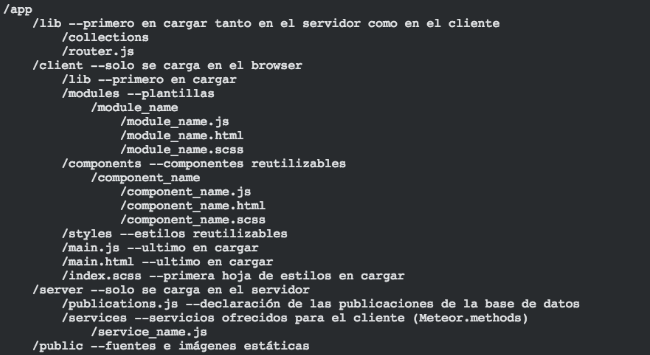
\includegraphics[width=1\textwidth]{hierarchyFolders.png}
    \caption{jerarqu�a de carpetas}
    \label{fig:hierarchyFolders}
\end{figure}

\paragraph{}
La carpeta \emph{/lib} de m�s alto nivel dentro de la jerarqu�a contiene todos los \emph{ficheros comunes} a ambos entornos (cliente y servidor) y es la primera en cargar. \emph{/server} y \emph{/client} contienen todos los \emph{ficheros ejecutables} por el servidor y por el cliente respectivamente. Dentro de cada una de las carpetas anteriores existe un orden de carga. Si poseen carpeta \emph{/lib} ser� la primera en cargar, despu�s es el turno de los dem�s ficheros en \emph{orden alfab�tico} y, por �ltimo, los ficheros \emph{main.*} sea cual sea su extensi�n. En la carpeta \emph{/public} se encuentra el \emph{contenido est�tico} de nuestra aplicaci�n (fuentes, im�genes, etc).

\paragraph{}
Como podemos ver seg�n el orden y �mbito de ejecuci�n Meteor ofrece un \emph{entorno de ejecuci�n sim�trico} (se ejecuta tanto en el cliente como en el servidor) dentro de la carpeta \emph{/lib} de m�s alto nivel en la jerarqu�a. La principal ventaja de esto es que no tenemos porqu� replicar c�digo. Podemos crear \emph{constructores} y dem�s funcionalidad necesaria en ambos entornos una sola vez y Meteor se encarga de saber que cargar en cada uno.
\paragraph{}
Adem�s, al ser MeteorJS una plataforma de desarrollo, no es necesario un \emph{gestor de tareas} como \textbf{GruntJS}\footnote{\url{http://gruntjs.com/}} o \textbf{GulpJS}\footnote{\url{http://gulpjs.com/}}. Estos se encargan de \textbf{automatizar tareas} tales como establecer la carga de ficheros sobre el  \emph{documento HTML}, \emph{minificar} todos los ficheros, establecer la \emph{configuraci�n del servidor} o arrancar nuestra aplicaci�n. Meteor posee un \textbf{CLI} (Interfaz de l�nea de comandos) que mediante el comando \emph{meteor} ya se encarga de establecer las configuraciones iniciales, cargar todos los ficheros seg�n el orden descrito e incluirlos en el documento y arrancar nuestro servidor. El \emph{minificado} no es necesario en un primer momento, puesto que con el \emph{deploying} (despliegue) se realizar�. Existen una gran cantidad de paquetes y constructores que lo har�n de forma autom�tica. 

\section{MongoDB}
\emph{MongoDB}\cite{bazMongoDB} es una base de datos \textbf{no relacional} cuya arquitectura \emph{se basa en documentos}. Al no ser \emph{relacional} como \textbf{mySQL}, \textbf{Oracle} o \textbf{PostgreeSQL} carece de \emph{claves primarias}. No hay que declarar un \emph{modelo de datos} puesto que lo que se almacenan son objetos en formato \textbf{BSON}\footnote{\url{http://bsonspec.org/}} (Binary JSON\footnote{\url{https://es.wikipedia.org/wiki/JSON}}) en el que todos los \emph{atributos} pueden ser utilizados como \emph{clave} a la hora de realizar b�squedas. Cada vez que un documento es insertado se le asocia un \emph{�ndice �nico}. Aunque no sea relacional ofrece la posibilidad de realizar un dise�o de este tipo. Esto es enlazando objetos pertenecientes a \emph{colecciones} (tablas) diferentes mediante su identificador o cualquier atributo v�lido. La gran ventaja de utilizar este tipo de base de datos es la \textbf{rapidez de acceso}. Como cualquier \emph{objeto javascript} un documento puede \emph{embeber} otros documentos (objetos) a los que se les puede establecer un �ndice y realizar \textbf{b�squedas indexadas}. Adem�s \emph{MongoDB} cuenta con m�dulos como \emph{\$agregation} que permite establecer reglas para cada colecci�n que permiten realizar b�squedas m�s complejas como por ejemplo establecer para qu� campo del documento se realiza una b�squeda mediante \emph{expresiones regulares}. 
\paragraph{}
Debido a que es una base de datos no relacional podemos \emph{embeber entidades} que dependan de otras en �stas. De no hacerlo as� el proceso de \emph{borrado de datos} hay que tomarlo con calma debido a que este tipo de base de datos no posee \textbf{joins} ni de herramientas que hagan que la \textbf{atomicidad} de los datos se mantenga como ocurre en las bases de datos relacionales. Aunque si queremos tambi�n realizar un dise�o desde un enfoque m�s limpio deber�amos de separar todas las entidades.

\subsection{MongoDB y MeteorJS}
\paragraph{}
Al crear una aplicaci�n mediante el CLI de MeteorJS directamente se crea una base de datos MongoDB. Aunque Meteor no trabaja con otro tipo de base de datos en un principio, se puede cambiar mediante la instalaci�n de paquetes. En la actualidad existen paquetes de bases de datos relacionales para Meteor que poseen reactividad y es este principio en el que se basa 
Meteor. 
\paragraph{}
Las tablas creadas en MongoDB en Meteor se convierten en colecciones, un wrapper para ofrecer funcionalidad desde la aplicaci�n y dotarlas de reactividad (las convierte en fuentes reactivas). Este objeto en el que se engloba a la tabla o entidad ofrece los m�todos \emph{.find()}, \emph{findOne()}, \emph{update()}, \emph{remove()}, \emph{insert()}, \emph{allow()} y \emph{deny()} que son los m�s usados. Hay que tener en cuenta que las colecciones en Meteor se declaran en la carpeta \emph{/lib}, cuyo contenido ser� ejecutado tanto en el entorno del cliente como en el del servidor. Esto quiere decir que cada entorno tendr� una instancia de cada colecci�n y esto al igual que es ventajoso en cuanto a rapidez en el cliente (puede acceder a la base de datos directamente "miniMongo" ), es peligroso por el mismo motivo. Para ello existen los m�todos \emph{deny()} y \emph{allow()} que establecen qu� operaciones sobre la colecci�n est�n permitidas en el cliente y cu�les no. 
\paragraph{}
Lo m�s sensato es permitir insertar y denegar el permiso para realizar cualquier alteraci�n sobre otros documentos ya presentes, al menos directamente. Para ello se usa el m�dulo methods de Meteor que permite configurar m�todos a los que llamar desde el cliente (tambi�n se declaran en la carpeta \emph{/lib}) y que se ejecutan en el servidor (donde no existe ning�n tipo de restricci�n).

\subsection{Publicaciones y Subscripciones}
\paragraph{}
Puesto que las instancias de las colecciones se encuentran accesibles tambi�n en el cliente debe haber un control sobre el contenido de las mismas dentro de MiniMongo. Para ello se utilizan las publicaciones y las subscripciones.
Las publicaciones se realizan en el lado del servidor y el cliente se subscribe a ellas. La moneda de cambio son los cursores. Un cursor es una fuente reactiva que engloba uno, varios o ning�n documento procedente de una colecci�n. El cliente al subscribirse a una publicaci�n obtiene el cursor y este lo transforma en documentos que se almacenan dentro de MiniMongo donde tendr� accesibles los documentos. Lo bueno de esto es que como se ha dicho los cursores son fuentes reactivas, esto quiere decir que en el momento que se produzca alg�n cambio que altere el cursor al que se est� subscrito, la publicaci�n cambiar� y la subscripci�n se actualizar�. Para aprovecharse de este fen�meno el cliente necesita extraer un cursor procedente de MiniMongo mediante \emph{NombreColecci�n.find()} o \emph{NombreColecci�n.findOne()} y asociarlo a un helper dentro de la l�gica de la plantilla.


\section{HTML5 Media}
Con la llegada y estandarizaci�n de HTML5 cada vez se trabaja m�s en herramientas que faciliten la comunicaci�n entre usuarios y que, en definitiva, brinden servicios interactivos a los mismos en tiempo real. Una de esas herramientas es \textbf{WebRTC} \cite{baz1} (Web Real-Time Communication).
\subsection{WebRTC}
Se trata de una API creada para permitir realizar llamadas de voz, chat de video e intercambio de archivos \textbf{P2P} (Peer to Peer) sin la necesidad de \emph{plugins}. Es \textbf{Open Source} (C�digo abierto). Fue creado primero por Google y la W3C se encarga ahora de su estandarizaci�n. Su desarrollo est� en proceso, por lo que se comporta de manera inestable en su funcionalidad avanzada.
Los navegadores que la soportan son Chrome, Firefox y Opera hoy en d�a. Esto se debe a que su m�dulo \textbf{navigator} facilita el acceso a los recursos media del ordenador (micr�fono, webcam).
\subsection{RTCRecorder}
Se trata de una API \cite{baz2} basada en WebRTC que proporciona una serie de herramientas para grabar video y audio de manera sencilla y pudiendo exportar el archivo creado y almacenarlo tanto en servicios cloud como en local. El creador de esta API tambi�n ha desarrollado otros m�dulos basados en WebRTC capaces por ejemplo de grabar video y audio sobre un elemento canvas. Hablaremos de esta API m�s adelante puesto que ha sido integrada en el proyecto.
\section{AceEditor}
\paragraph{}
\textbf{AceEditor}\cite{AceEditor} es una API que permite transformar un contenedor HTML (por ejemplo un \emph{$<$div$>$}) en un editor de texto completo. Adem�s proporciona una serie de m�todos que permiten personalizarlo y \emph{capturar eventos} que se produzcan en dicho editor. Existen otras APIs parecidas como \textbf{CodeMirror}\footnote{\url{https://codemirror.net/}}, pero �sta posee m�s documentaci�n y est� disponible como paquete para Meteor \cite{AceEditorPackage}. Exploraremos m�s a fondo esta API m�s adelante.
\section{Tecnolog�as Cloud}
\paragraph{}
Hoy en d�a el t�rmino \emph{Cloud} est� muy extendido. La mayor�a de aplicaciones y sitios web utilizan tecnolog�as cloud para almacenar grandes cantidades de datos y liberar memoria propia de la aplicaci�n o bien son utilizadas como base de datos. Ejemplos de tecnolog�as cloud son \textbf{Google Drive}, \textbf{Dropbox}, \textbf{Youtube}, \textbf{Amazon S3}, \textbf{Soundcloud}, \textbf{mLab} o \textbf{DigitalOcean}.
\paragraph{} La mayor�a de los anteriores son utilizados como servicios cloud extra o para almacenar contenidos de la aplicaci�n (ficheros, im�genes, audios, videos). Amazon S3 o mLab son utilizados como base de datos de la aplicaci�n y su ventaja radica en que, a la hora de realizar el despliegue, utilizamos servidores externos en los que almacenaremos la base de datos de nuestra aplicaci�n.
\subsection{API Soundcloud}
Soundcloud\footnote{\url{https://soundcloud.com}} es un sitio web que permite alojar archivos de audio al estilo de Youtube con v�deos. Posee un API disponible en diferentes lenguajes de programaci�n como Ruby, javascript y PHP para realizar peticiones REST y por tanto un espacio para desarrolladores en el cual crear diferentes aplicaciones con las que comunicarse la API. Se trata de una soluci�n factible a la hora de desarrollar un proyecto peque�o ya que tiene limitaciones en lo que respecta a espacio. Si nos encontramos ante un proyecto de gran envergadura necesitaremos explorar otras v�as como \textbf{GridFS}\footnote{\url{https://docs.mongodb.com/manual/core/gridfs/}} aplicado a otro servicio cloud de base de datos como Amazon S3.  
\paragraph{} 
Tambi�n proporciona herramientas de \textbf{Streaming} de gran utilidad a la hora de reproducir dichos archivos de audio en nuestra aplicaci�n de forma remota.
\paragraph{}
Exploraremos a fondo esta API puesto que es una de las herramientas m�s importantes incluidas en este proyecto.

\section{Herramientas para trabajo en equipo}
El mundo del desarrollo web es altamente competitivo y como tal exige la obtenci�n de resultados muy a corto plazo. Para conseguir este objetivo surgen las metodolog�as �giles como \textbf{SCRUM}\footnote{\url{https://en.wikipedia.org/wiki/Scrum_(software_development)}} que, seg�n su definici�n, no es m�s que un proceso en el que se aplican una sucesi�n de buenas pr�cticas para trabajar en equipo. La finalidad es conseguir un equipo altamente productivo. La base de esta metodolog�a es la realimentaci�n o feedback, es decir, es un proceso circular compuesto por varias fases y realimentado en el cual el cliente toma conciencia de cada ciclo aportando sus cr�ticas. 
\paragraph{}
Para reforzar este proceso y facilitar la labor del desarrollador y de todo el equipo existen distintas herramientas como \textbf{GitHub}, \textbf{PivotalTracker} y \textbf{Slack} entre otras. Estas herramientas han sido utilizadas a lo largo de este proyecto.
\subsection{Git y GitHub}
\paragraph{}
Git es el sistema de control de versiones m�s usado en el mundo del desarrollo. Crea una copia del proyecto en un \textbf{repositorio} y a trav�s de sus \textbf{commits} se almacenan versiones recuperables del mismo. Incorpora un sistema para generar \textbf{ramas} de versiones que posteriormente pueden volver a unirse para conformar el resultado final del proyecto o finalizar alguna fase. Esto lo hace verdaderamente potente a la hora de utilizarlo en grupo y por tanto es necesario compartir el repositorio entre los integrantes del equipo de desarrollo. Esto se hace mediante GitHub, una plataforma en la que almacenar proyectos p�blicos o privados que integra el sistema de control de versiones mencionado anteriormente. Permite la copia de cualquier versi�n desde un usuario a otro (\textbf{fork}) y puede desarrollarse un seguimiento de todo el proyecto mediante el espacio para \textbf{Wiki}.
\paragraph{}
Adem�s permite la sincronizaci�n de otros servicios afines al proyecto como PivotalTracker.
\subsection{PivotalTracker}
La primera fase de toda metodolog�a �gil en un proyecto de desarrollo se basa en el \emph{an�lisis} y la \emph{extracci�n de requisitos}. Estos requisitos son llamados \textbf{historias de usuario} y son el elemento base de PivotalTracker. 
\paragraph{}
PivotalTracker es una plataforma de organizaci�n de proyectos mediante tareas o items a completar. Cada historia de usuario normalmente es dividida en distintas tareas. Una vez creado un proyecto en esta plataforma y establecido los miembros comienza la asignaci�n de tareas. Se establecen diferentes espacios o ambientes de trabajo que indican la prioridad de las tareas (\emph{Icebox}, \emph{current}, \emph{done}, etc). Con la creaci�n de cada tarea viene la estimaci�n del tiempo de trabajo de la misma y a mayor valor de estimaci�n m�s miembros la tendr�n asignada. Una vez finalizada la tarea es necesaria la validaci�n de la misma por el resto del equipo. De esta manera est� asegurado el correcto desarrollo del proyecto.
\subsection{Slack}
Slack es una plataforma de comunicaci�n destinada a grandes proyectos. Se organiza mediante \textbf{canales} y permite el intercambio de ficheros, informaci�n y mucho m�s a trav�s de \textbf{chat}. Adem�s ofrece la posibilidad de vincular cada canal a los servicios utilizados en el proyecto como GitHub y PivotalTracker por lo que cada acci�n y avance quedar� reflejado y notificado a los miembros del equipo.
Se trata de una herramienta muy �til para el trabajo en remoto y como \emph{historial de proyecto}.
\section{Contenidos}
En esta secci�n se enuncian los contenidos y la organizaci�n de la informaci�n en esta memoria. A saber:
\begin{itemize}
\item \textbf{Cap�tulo 3: } en este cap�tulo se ha pretendido presentar la motivaci�n de realizar este proyecto, la metodolog�a que se ha llevado a cabo y el plan de trabajo que se ha desarrollado a lo largo del mismo.
\item \textbf{Cap�tulo 4: } en �l se detalla el proceso de dise�o y desarrollo. Se ha organizado en funci�n de los prototipos de los que consta este proyecto.
\item \textbf{Cap�tulo 5: } se presentan las pruebas de validaci�n realizadas. Exponiendo su planteamiento, dise�o, proceso y an�lisis.
\item \textbf{Cap�tulo 6: } en �l se describen las conclusiones extra�das una vez finalizado el proyecto y a la luz de los resultados obtenidos.
\item \textbf{Cap�tulo 7: } aqu� se detalla la bibliograf�a del proyecto. Engloba sitios oficiales, tutoriales, documentaci�n de APIs usadas y la propia documentaci�n del mismo.
\item \textbf{Ap�ndices: } esta apartado est� compuesto por cuatro cap�tulos y su finalidad es servir de apoyo al lector de esta memoria.
\end{itemize}
\chapter{Objetivos y metodolog�a}\label{ch:metodologia}
En este cap�tulo se expone el problema que impulsa la motivaci�n de realizar este proyecto, los objetivos y requisitos marcados, la metodolog�a elegida para su desarrollo y el plan de trabajo llevado a cabo adoptando dicha metodolog�a. Adem�s se enumeran tecnolog�as que sirven de inspiraci�n al mismo.
\section{Motivaci�n}
\paragraph{}
En la actualidad existen distintas aplicaciones y sitios web destinados a facilitar la labor del desarrollador. Sitios como PivotalTracker, Github, \textbf{GitBucket}, \textbf{CodePen}, \textbf{Codecademy}, \textbf{StackOverflow} o \textbf{StackExchange}\footnote{\url{http://stackexchange.com/}}. Estos sitios proporcionan herramientas para un correcto desarrollo de cualquier proyecto. En el caso de Github o GitBucket facilitan la creaci�n de repositorios remotos con un sistema de control de versiones. PivotalTracker permite organizar las tareas de un proyecto y CodePen, Codecademy y StackOverflow son sitios web para el aprendizaje y compartir conocimientos. 
\paragraph{}
Es precisamente el \emph{aprender y compartir} lo que mueve el mundo del desarrollo. Cualquier desarrollador utiliza ideas propias y de otros desarrolladores para realizar cualquier proyecto. Pero muchas veces esas ideas no son muy intuitivas o f�ciles de aprender a partir de un art�culo o un fichero de c�digo completado. Por esto muchas veces recurrimos a \emph{plataformas de difusi�n de video} para poder aprender r�pidamente. 
\paragraph{}
Tambi�n existen otros sitios web cuya finalidad es la de compartir conocimientos y aprender de forma interactiva como \textbf{Mediathread}\footnote{\url{http://mediathread.ccnmtl.columbia.edu/accounts/login/?next=/}}, \textbf{YourTalk}\footnote{\url{http://urtalk.com/about/}} y \textbf{KhanAcademy}\footnote{\url{https://www.khanacademy.org/computing/computer-programming/html-css-js/html-js-dom-animation/p/animating-dom-with-setinterval}}. Este proyecto intenta emular dicha funcionalidad e ir un paso m�s all�.
\paragraph{}
De esta necesidad surge la motivaci�n de crear una \textbf{aplicaci�n web} que sirva de \textbf{plataforma para todos los desarrolladores}. Una plataforma donde puedan \textbf{aprender} r�pidamente, \textbf{intercambiar} conocimientos de manera \textbf{interactiva} y que permita la \textbf{comunicaci�n} entre sus usuarios. Puesto que la informaci�n deber�a ser lo m�s visual e interactiva posible el formato se basar� en \textbf{grabaciones de c�digo y audio sobre un editor}. Adem�s Cada grabaci�n podr� pausarse y crear una nueva a modo de respuesta a partir de ese instante.
\section{Objetivos}\label{sec:objetivos}
Como resultado del an�lisis motivaci�n descrita, podemos extraer una serie de objetivos generales que deben de cumplirse en la implementaci�n de este proyecto. Estos objetivos son: 
\begin{enumerate}
\item Desarrollar una aplicaci�n funcional y que sirva de herramienta para los desarrolladores en tiempo real.
\item La aplicaci�n debe ser atractiva al usuario e intuitiva atendiendo a las bases UX (User Experience) m�s importantes.
\item La aplicaci�n debe ser fluida y estar optimizada. 
\item La aplicaci�n debe constituir una herramienta did�ctica cuyo elemento de informaci�n base sea visual e interactivo.
\end{enumerate}
\section{Requisitos}\label{sec:requisitos}
\paragraph{} 
Con la motivaci�n surge el proceso de pensar en las necesidades que tendr� el usuario al utilizar la aplicaci�n. Estas necesidades se traducen en requisitos que debe cumplir la aplicaci�n y que hay que tener presentes en todo momento del dise�o y del desarrollo. Tanto nuestro concepto de la aplicaci�n como las necesidades del usuario pueden verse alteradas durante el desarrollo del proyecto por lo tanto pueden surgir nuevos requisitos y verse alterados los ya establecidos.
\paragraph{}
A continuaci�n se exponen todos los requisitos que deber�a cumplir nuestra aplicaci�n y que se han ido extrayendo a lo largo de la realizaci�n del proyecto:
 \begin{itemize}
 \item \textbf{Experiencia: }\label{rExp}
	\begin{enumerate}
		\item \label{r19} Para una mejor experiencia es necesario que el usuario conozca lo que sucede dentro de aplicaci�n para ello debe existir un m�dulo que permita crear notificaciones personalizadas y de inter�s para el usuario. 
		\item \label{r20} El usuario deber� tener acceso r�pido a las listas de contenido.
		\item \label{r23} La aplicaci�n deber� ser �ptima y precisa y proporcionar al usuario una interfaz cuidada e intuitiva.
		\item \label{r61} Para una mejor experiencia es necesario realizar al usuario recomendaciones de contenido basadas en sus gustos y su recorrido dentro de la aplicaci�n.

		\item \label{r62} Para una mejor experiencia es necesario mostrar al usuario las tendencias o el contenido m�s popular dentro de la aplicaci�n.

		\item \label{r63} Para una mejor experiencia es necesario aportar al usuario un mini tutorial compuesto por tareas b�sicas que le ayude a dar sus primeros pasos en la aplicaci�n.
		\item \label{r64} Es necesario que los usuarios puedan explorar una descripci�n de las caracter�sticas de la aplicaci�n para ello se debe crear un espacio en el que el usuario las conozca.

		\item \label{r65} Es necesario que los usuarios puedan aprender c�mo usar la aplicaci�n para ello se debe crear un espacio con tutoriales.
		\item \label{r69} Es necesario que los usuarios puedan recibir notificaciones de nuevos mensajes de sus conversaciones abiertas cuando no est�n visualizando dicha conversaci�n.
	\end{enumerate}
 \item \textbf{Registro: }\label{rReg}
 	\begin{enumerate}
	 	\item \label{r1} Se deber� proporcionar una interfaz de inicio para que el usuario pueda explorar las caracter�sticas de la aplicaci�n, aprender, y poder crear un usuario para acceder a la misma.
		\item \label{r2} Los usuarios deben ser autenticados para poder acceder a la mayor�a de la funcionalidad de la aplicaci�n.

		\item \label{r3} Un usuario podr� registrarse introduciendo un nombre de usuario, un correo electr�nico y una contrase�a o bien mediante los servicios integrados de 
Facebook, Github y Google+.
		\item \label{r6} Un usuario podr� acceder a la aplicaci�n introduciendo su nombre de usuario o email asociado y su contrase�a.
		\item \label{r5} Un usuario podr� recuperar su contrase�a siempre que tenga asociado un correo electr�nico y �ste haya sido verificado y puede estar autenticado o no.
	\end{enumerate}

 \item \textbf{Servicios: }\label{rServ}
 	\begin{enumerate}
		\item \label{r4} Es necesario proporcionar al usuario un proceso de validaci�n o verificaci�n de email, un proceso de cambio de contrase�a y otro de recuperaci�n de la misma.
		\item \label{r89} Los emails no son entidades dentro de la aplicaci�n. No se guarda registro de ellos. Simplemente se proporciona una herramienta que permite su redacci�n y env�o.
	\end{enumerate}

 \item \textbf{Perfil: }\label{rProf}
 	\begin{enumerate}
		\item \label{r8} Un usuario podr� realizar peticiones de contacto a otros usuarios para a�adirlos a su lista de contactos.
		\item \label{r9} Un usuario podr� aceptar o rechazar peticiones. 

		\item \label{r10} Un usuario podr� reenviar una solicitud de contacto que haya sido rechazada.
		\item \label{r70} Cada usuario deber� poder acceder a toda su informaci�n y contenido. Para ello se les proporcionar� un enlace en todo momento a su perfil y un acceso a sus contenidos principales.

		\item \label{r71} Cada usuario podr� visualizar la lista de sus contenidos, sus subscripciones, sus conversaciones, una lista con las �ltimas reproducciones y sus contactos.

		\item \label{r72} Cada usuario podr� editar su perfil a saber: su avatar, el banner, su descripci�n y sus emails.

		\item \label{r73} Los perfiles podr�n ser vistos por todos los usuarios por lo que se establecen dos roles: propietario, visitante.

		\item \label{r74} Un visitante ya sea contacto o no del propietario podr� visualizar todo su contenido a excepci�n de sus conversaciones.

		\item \label{r75} Un visitante ya sea contacto o no del propietario podr� acceder al perfil asociado al servicio integrado en el caso de que el propietario se haya registrado mediante dicho servicio.

		\item \label{r76} Un visitante que sea contacto del propietario podr� iniciar una conversaci�n o redactar un email al email del propietario en el caso de que �ste tenga configurado y verificado alg�n correo.

		\item \label{r77} Un visitante que no sea contacto podr� enviar una solicitud de contacto al propietario.

		\item \label{r78} Se debe crear un espacio para realizar solicitudes de contacto que lo componga un buscador (autocompletado de usuarios) y listas de peticiones recibidas y enviadas y su estado.
	\end{enumerate}

 \item \textbf{Contenidos:}\label{rCont}
 	\begin{enumerate}
		\item \label{r7} Un usuario podr� crear canales, lecciones, grabaciones y conversaciones.
		\item \label{r12} Cualquier contenido se podr� etiquetar para facilitar la recomendaci�n y b�squeda del mismo, con la excepcion de las conversaciones.

		\item \label{r13} Cualquier contenido se podr� votar y comentar con la excepci�n de las conversaciones.

		\item \label{r14} Se podr�n crear respuestas a los comentarios.

		\item \label{r15} Todo contenido deber� mostar contadores de votos, subcontenidos y usuarios subscritos (cuando proceda).

		\item \label{r16} Todo contenido podr� ser editado.

		\item \label{r17} Todos los contenidos podr�n ser borrados a excepci�n de las conversaciones.

		\item \label{r18} No se podr� borrar ning�n contenido con subcontenidos.
		\item \label{r21} Todas las listas de contenido podr�n ser filtradas por dos tipos de filtros: m�s recientes y m�s populares.
		\item \label{r22} Para todo tipo de contenido existen dos roles con un tipo de acceso diferente a las funcionalidades propias del mismo.
		\item \label{r66} Es necesario que los contenidos puedan mostrarse en listas para su navegaci�n. Para ello cada contenido debe poseer una miniatura asociada que muestre la informaci�n m�s relevante para cada tipo de contenido.

		\item \label{r67} Es necesaria la presencia de un buscador de contenido dentro de la aplicaci�n.

		\item \label{r68} Las b�squedas en la aplicaci�n ser�n din�micas y con un sistema de etiquetas que se ir�n sugiriendo de manera autom�mica.
	\end{enumerate}
	
\item \textbf{Grabaciones: }\label{rRec}
 	\begin{enumerate}
		\item \label{r24} Las grabaciones ser�n grabaciones de c�digo y audio sobre editor.

		\item \label{r25} Las grabaciones ser�n el elemento at�mico en lo que respecta a contenido dentro de la aplicaci�n.

		\item \label{r26} El objeto de cada grabaci�n ser� grabar documentos de c�digo. 

		\item \label{r27} Cada grabaci�n podr� tener 1 o m�s documentos.

		\item \label{r28} Los documentos tendr�n un titulo �nico dentro de cada grabaci�n, un modo (lenguaje en el que est�n programados) y un tema (aspecto en el editor).

		\item \label{r29} Un usuario podr� crear grabaciones.

		\item \label{r30} Un usuario podr� crear respuestas sobre cualquier grabaci�n a partir de cualquier instante de su reproducci�n.

		\item \label{r31} Las grabaciones podr�n ser aisladas o pertenecer a un canal o lecci�n.

		\item \label{r32} El usuario podr� navegar, visualizar y reproducir cualquier grabaci�n.

		\item \label{r33} El usuario podr� acceder al padre de una grabaci�n (respuesta) desde la p�gina de visualizaci�n de la misma.

		\item \label{r34} El usuario podr� visualizar tanto las respuestas a una grabaci�n c�mo grabaciones relacionadas a la misma.

		\item \label{r35} El usuario podr� acceder al canal o lecci�n a la que pertenece cualquier grabaci�n.

		\item \label{r36} Las grabaciones no tienen porqu� poseer un t�tulo �nico, pero s� deben tener uno. Opcionalmente tendr�n una descripci�n y una lista de etiquetas.

		\item \label{r37} Las grabaciones podr�n ser editadas mediante una respuesta.

		\item \label{r38} El usuario podr� cambiar el instante de la reproducci�n, pausarla o reanudarla.
	\end{enumerate}
	
\item \textbf{Canales: }\label{rChan}
 	\begin{enumerate}
		\item \label{r39} Un usuario podr� crear canales.

		\item \label{r40} Un usuario podr� subscribirse a cualquier canal que no haya sido creado por �l mismo para recibir notificaciones relevantes.

		\item \label{r41} El contenido de los canales estar� formado por una lista de grabaciones.

		\item \label{r42} La creaci�n de contenido no est� restringida para los canales. Todos los usuarios podr�n generar contenido dentro de cualquier canal.

		\item \label{r43} Cualquier usuario podr� votar y comentar canales y sus contenidos.

		\item \label{r44} Cada canal podr� ser editado por el creador.
	\end{enumerate}

 

 \item \textbf{Lecciones: }\label{rLess}
 	\begin{enumerate}
		\item \label{r45} Un usuario podr� crear lecciones.

		\item \label{r46} El contenido de las lecciones ser�n secciones formadas por una lista de grabaciones.

		\item \label{r47} La creaci�n de contenido estar� restringida para las lecciones. S�lo el creador de la lecci�n puede crear contenido directo a las mismas a saber: secciones y grabaciones.

		\item \label{r48} Un usuario podr� subscribirse a cualquier lecci�n que no haya sido creada por �l mismo para poder acceder a su contenido y recibir las notificaciones relevantes.

		\item \label{r49} Cualquier usuario subscrito a una lecci�n podr� crear respuestas a todas las grabaciones que existan dentro de la misma.

		\item \label{r50} El contenido de una secci�n se reproducir� mediante el concepto de lista de reproducci�n. 

		\item \label{r51}  El reproductor deber� identificar si la grabaci�n procede de una lecci�n y si forma parte de una lista de reproducci�n. Si es el caso deber� proporcionar una interfaz para navegar por la lista de reproducci�n y establecer opciones tipo: reproducci�n y repetici�n autom�tica.

		\item \label{r52} Las opciones reproducci�n y repetici�n autom�tica estar�n asociadas al usuario no a la secci�n.

		\item \label{r53} La reproducci�n autom�tica provocar� que se reproduzca la siguiente grabaci�n de la lista al finalizar la actual.

		\item \label{r54} La repetici�n autom�tica provocar� que la reproducci�n de la lista sea circular (ni principio ni fin).

		\item \label{r55} Cualquier usuario que est� subscrito a una lecci�n podr� votar a la misma y a sus contenidos (grabaciones).

		\item \label{r56} Cualquier usuario que est� subscrito a una lecci�n podr� comentar la misma y sus contenidos (grabaciones).

		\item \label{r57} Cada lecci�n podr� ser editada por el creador. 

		\item \label{r58} El orden de las secciones podr� ser cambiado por el creador.

		\item \label{r59}  El orden de las grabaciones que forman una secci�n podr� ser cambiado por el creador.

		\item \label{r60} Las secciones podr�n ser borradas por el creador en cualquier momento, siempre que no tengan contenido.
	\end{enumerate}
\item \textbf{Conversaciones: }\label{rConv}
	\begin{enumerate}
		\item \label{r11} Un usuario podr� crear conversaciones con otros usuarios que est�n en su lista de contactos.
		\item \label{r79} Una conversaci�n debe incluir al menos 2 contactos en el momento de creaci�n. 

		\item \label{r80} Cada conversaci�n podr� ser editada por todos los miembros. 

		\item \label{r81} Las opciones de edici�n de cada conversaci�n est�n restringidas seg�n roles: creador o l�der, invitados.

		\item \label{r82} S�lo el l�der de la conversaci�n puede cambiar el asunto y expulsar a miembros de la misma.

		\item \label{r83} El l�der s�lo podr� dejar la conversaci�n si antes ha nombrado como nuevo l�der a alguno de los miembros invitados.

		\item \label{r84} Todos los invitados podr�n dejar la conversaci�n en el momento que deseen.

		\item \label{r85} Todos los miembros podr�n eliminar el historial de mensajes.

		\item \label{r86} Todos los miembros podr�n invitar a la conversaci�n a usuarios que sean sus contactos.

		\item \label{r87} Todos los miembros podr�n cambiar el fondo de la conversaci�n y dicha configuraci�n estar� asociada a dicho usuario.

		\item \label{r88} Las conversaciones son privadas, es decir, ning�n usuario puede acceder a ninguna conversaci�n de la que no sea miembro aunque alguno de sus contactos sea miembro.
	\end{enumerate}
\end{itemize}

 
\section{Metodolog�a y plan de trabajo}
\subsection{Metodolog�a}
En este Trabajo Fin de Grado hemos seguido una metodolog�a de \textbf{realimentaci�n} o \textbf{feedback} basada en la metodolog�a �gil \textbf{SCRUM}. Se basa en que el producto final es el resultado de una serie de \textbf{prototipos} los cuales han sido implementados en cada \emph{iteraci�n} del proceso. Podemos ver las etapas de cada iteraci�n en la figura \ref{fig:metodologia} a saber: extracci�n de requisitos, aprendizaje, etapa de dise�o, etapa de desarrollo, realizaci�n de pruebas y evaluaci�n del producto.

\begin{figure}[h]
\centering
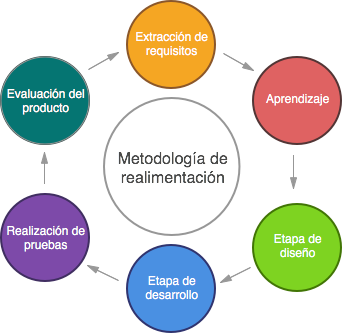
\includegraphics[scale=0.65]{fbackM.png}
\caption{Esquema metodolog�a de realimentaci�n}
\label{fig:metodologia}
\end{figure}


\subsection{Plan de trabajo}
El c�digo fuente de este TFG est� disponible en un repositorio p�blico en GitHub \cite{bazGitRepo} y se ha ido documentando en la Wiki \cite{bazWikiProyect} del mismo. La documentaci�n incluye manuales de uso de los m�dulos principales desarrollados, dise�o de los objetos en la base de datos y un historial descriptivo de las reuniones realizadas con el tutor. La comunicaci�n con el tutor se ha realizado mediante la plataforma Slack y a trav�s de PivotalTracker se han ido estableciendo y completando las diferentes tareas de cada fase del desarrollo del proyecto.
\paragraph{}
El plan de trabajo se ha desarrollado en las siguientes fases:  
\begin{itemize}
\item \textbf{Fase1 - Consolidaci�n, b�squeda y aprendizaje}: esta fase corresponde al proceso de extracci�n de requisitos iniciales y consolidaci�n del concepto de la aplicaci�n, a la b�squeda de herramientas necesarias y al aprendizaje de dichas herramientas (MeteorJS, Javascript, HTML5, CSS3, SASS, WebRTC y RTCRecorder, APIs Soundcloud, AceEditor, IronRouter y dem�s paquetes). 
\item \textbf{Fase 2 - Prototipado:} esta fase ha sido la que m�s tiempo ha requerido y en la que se ha empleado la metodolog�a iterativa descrita anteriormente. En cada iteraci�n se ha enunciado y desarrollado un prototipo cuyo resultado ha servido de base al siguiente. Cada fase ha llevado consigo la realizaci�n de las siguientes tareas:
\begin{enumerate}
	\item Extracci�n de requisitos
	\item Extracci�n de entidades
	\item Dise�o de la base de datos
	\item Dise�o front-end e Interfaces de usuario
	\item Desarrollo de Interfaces
	\item Pruebas y evaluaci�n
\end{enumerate}
\item \textbf{Fase 3 - Final:} una vez implementado el prototipo final se ha procedido a la fase final del proyecto que corresponde a la mejora global y su despliegue. El despliegue implica tambi�n la introducci�n de licencias para preservar los derechos de autor y convertir el c�digo en c�digo libre.
\end{itemize}

\paragraph{}
En el siguiente cap�tulo se describe detalladamente el dise�o y desarrollo de cada los prototipos m�s relevantes que se han implementado a lo largo del proyecto.







%%%%%%%%%%%%%%%%%%%%%%%%%%%%%%%%%%%%%%%%%%%%%%%%%%%%%%%%%%
%%%%%%%                  															       %%%%%%
%%%%%%%                                      CAPITULO 3: DISE�O DE LA APLICACI�N                                   %%%%%%
%%%%%%%  																	       %%%%%%
%%%%%%%%%%%%%%%%%%%%%%%%%%%%%%%%%%%%%%%%%%%%%%%%%%%%%%%%%%
\chapter{Dise�o de la aplicaci�n}
\paragraph{}
El primer paso a la hora de desarrollar cualquier aplicaci�n es el dise�o de la misma. Este proceso engloba tanto el dise�o visual como la elecci�n de herramientas a utilizar seg�n los requisitos de dicha aplicaci�n. En este cap�tulo se expone todo lo relacionado con este proceso.
\section{Tipo de arquitectura}
\paragraph{}
El modelo de arquitectura m�s habitual es el \textbf{MVC} (Modelo Vista Controlador) (figura \ref{fig:mvcpattern}). El modelo corresponder�a con la arquitectura de base de datos y el dise�o de la misma, la vista son las interfaces o plantillas que se muestran al usuario y el controlador es el encargado de dotar a la aplicaci�n de l�gica y funcionalidad. Existen otros tipos de arquitectura tales como \textbf{MVVM} (figura \ref{fig:mvvmpattern}), donde el controlador del patr�n MVC se sustituye por VM o \emph{ViewModel} que establece que cada vista posee l�gica y un sistema de \emph{data-binding} entre plantillas.

\begin{figure}[htbp]
    \centering
    \subfigure[Patr�n de arquitectura MVC]{
   	 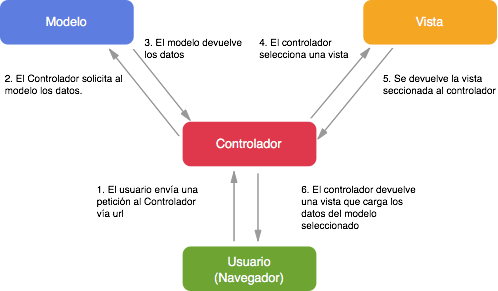
\includegraphics[width=1\textwidth]{mvc.png}
    	\label{fig:mvcpattern}
    }
    \subfigure[Patr�n de arquitectura MVVM]{
    	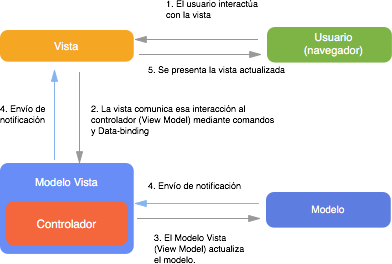
\includegraphics[width=1\textwidth]{mvvm.png}
	 \label{fig:mvvmpattern}
    }
    \caption{Patrones de arquitectura}
    \label{fig:patterns}
\end{figure}

\paragraph{}
La elecci�n del patr�n de arquitectura a usar es importante puesto que esa decisi�n nos limitar� a la hora de usar determinadas herramientas.
\paragraph{}
Meteor posee una arquitectura peculiar. En la documentaci�n se expone que posee una arquitectura MVC. Pero, dado que sus vistas poseen l�gica y existe data-binding el patr�n que seg�n mis conocimientos se basa es MVVM. Por este motivo el patr�n de arquitectura utilizado en esta aplicaci�n ser� el MVVM (Model View ViewModel).
\section{B�squeda de herramientas de desarrollo}
\paragraph{}
Partiendo de los requisitos establecidos que caracterizar�n la aplicaci�n podemos afirmar que necesitamos encontrar herramientas que nos permitan construir una aplicaci�n en tiempo real, realizar grabaciones de audio, una interfaz con UX como par�metro fundamental y que trabaje de manera �ptima.

\subsubsection{Aplicaci�n en tiempo real y prototipado r�pido}
\paragraph{}
Necesitamos alg�n framework o plataforma que trabaje con el concepto de reactividad o que lo simule. Elegimos MeteorJS por su flexibilidad y su asombroso concepto de reactividad. Al utilizar esta plataforma no tenemos que preocuparnos de qu� frameworks usar para desarrollar el cliente por un lado y el servidor por otro o como gestionar los modelos de datos porque Meteor ya incluye toda la l�gica necesario y seg�n su paradigma o patr�n de trabajo engloba ambos entornos. Adem�s no hay que declarar el modelo de datos de forma tradicional o como en otras plataformas y frameworks ya que Meteor incluye desde el principio MongoDB como su base de datos. 
\paragraph{}
Para el enrutamiento es precisa otra herramienta que nos proporcione la funcionalidad de especificar a qu� recurso pertenece una plantilla y que datos asociamos a ella. Para ello existen varios paquetes para Meteor que realizan este proceso como IronRouter o FlowRouter. Ambos igual de v�lidos pero para este proyecto se ha optado por IronRouter, ya que dispone de mayor documentaci�n.
\paragraph{}
Para el concepto de publicaciones y subscripciones de Meteor usaremos publishComposite, un paquete que permite realizar publicaciones compuestas (varias colecciones con relaci�n de dependencia reactiva) y que siguen manteniendo el principio de reactividad y optimizando nuestro sistema de subscripciones. Sin este paquete realizar esta labor es m�s compleja.  
\paragraph{}
Otro aspecto a tener en cuenta es la gesti�n de paquetes. En este �mbito Bower es excelente. Pero usando Meteor no lo necesitamos ya que posee su propio gestor de paquetes y mediante su CLI podemos a�adir, actualizar y borrar paquetes de nuestro proyecto.

\subsubsection{Grabaciones de audio}
\paragraph{}
La grabaci�n sobre editor con audio constituye el elemento base de esta aplicaci�n. Existen numerosas formas de grabar audio v�a web y algunas API de sitios como SoundCloud incorporan un grabador de audio directamente. Aunque esta hubiera sido la v�a m�s r�pida, la verdad es que no habr�a sido la m�s flexible, ya que el hacerlo de esta manera requer�a que el uploading se efectuara en SoundCloud. Por este motivo se ha utilizado la tecnolog�a de WebRTC para esta tarea y construido un grabador modular que puede incorporarse facilmente a otros proyectos y que adem�s si se desea usar el servicio de hosting de SoundCloud seguir�a siendo factible. 

\subsubsection{Interfaz con UX como par�metro de dise�o fundamental}
\paragraph{}
Toda aplicaci�n debe ser atractiva al usuario y no s�lo en t�rminos visuales sino en eficacia a la hora de gestionar acciones. Existen numerorsos frameworks y bibliotecas frontend para desarrollar dicha labor correctamente tales como Foundation, Bootstrap o Pure.css. En este proyecto nos hemos decantado por la biblioteca frontend Bootstrap, quiz� la m�s explotada hasta la fecha. Su sistema de maquetaci�n se ha convertido en est�ndar para el dise�o web. Tambi�n nos hemos visto con la necesidad de dotar de flexibilidad a las plantillas cuando el sistema de columnas de Bootstrap no mostraba los resultados deseados y para ello hemos utilizado la tecnolog�a Flexbox.
\paragraph{}
Hoy en d�a trabar con CSS o CSS3 puro se podr�a considerar un error, ya que existen preprocesadores que permiten una mejor arquitectura para nuestros estilos como son Less y Sass. Ambos son muy parecidos, aunque Sass es mucho m�s legible. Por ello se han desarrollado las hojas de estilos mediante este preprocesador utilizando un paquete.





\section{Dise�o entidades y base de datos}
\paragraph{}
Esta fase del dise�o es primordial pues sin unas entidades bien definidas no ser�a posible la organizaci�n del contenido del sitio ni su correcta presentaci�n. El dise�o de entidades se basa en las necesidades del usuario al utilizar la aplicaci�n y lo que queremos que dicha aplicaci�n le aporte. La base de datos ser� la traducci�n del modelo entidad relaci�n dise�ado a partir de las caracter�sticas de cada entidad y su relaci�n con las dem�s.

\subsection{Entidades}
\paragraph{}
Hemos dicho que las grabaciones en esta aplicaci�n son el elemento at�mico o base. Por lo que aqu� tenemos nuestra primera entidad de la aplicaci�n.
\paragraph{}
 Ahora hay que pararse a pensar y a hacernos preguntas del tipo �Qu� le gustar�a hacer al usuario con esas grabaciones?�C�mo estar�an organizadas?�Existen l�mites?�Cu�l es el fin de la grabaci�n?.
Esto nos lleva a crear un dise�o con un enfoque did�ctico y funcional, el cual corresponde con la finalidad de realizar cualquier grabaci�n. Por esto esta aplicaci�n lo que pretende es crear una Comunidad para desarrolladores y cualquiera que le interese el mundo del software. Cada usuario podr� compartir sus conocimientos y sus inquietudes, dudas en lo que a programaci�n se refiere. Vista esta dualidad debemos establecer dos �mbitos en la aplicaci�n. Uno corresponder�a con el aprendizaje y otro a la ense�anza. En definitiva se basa en el intercambio de conocimientos sobre software.
\paragraph{}
Por este motivo establecemos las entidades de Canal y de Lecci�n. El elemento canal debe estar basado en un tema espec�fico y cualquier usuario puede contribuir con sus conocimientos sobre el tema. Ser�a una especie de foro, pero con preguntas y respuestas propuestas mediante grabaci�n de audio sobre editor. El elemento lecci�n se diferencia del elemento canal en que s�lo el autor de dicho elemento puede generar contenido de forma directa. Este contenido se generar� y se organizar� en torno a secciones, una nueva entidad. Las secciones tendr�n un t�tulo y estar� compuestas de una o m�s grabaciones. Adem�s para una mejor experiencia de usuario estas grabaciones deber�n componer una lista de reproducci�n. Esta lista tendr� las opciones de reproducci�n autom�tica y de reproducci�n circular (al finalizar con la �ltima comenzar� con la primera de la lista). 
\paragraph{}
Las lecciones deben ser participativas. No es muy did�ctico que s�lo el creador de la lecci�n sea el que comparta sus conocimientos. Aunque s� que es verdad que los contenidos inmediatos de la lecci�n s�lo son creados por el autor, esos contenidos pueden ser respondidos o corregidos mediante una nueva grabaci�n que no formar� parte de la secci�n pero que s� quedar� almacenada en la lista de respuestas de dicha grabaci�n inicial. Con esto surge la necesidad de que a cada grabaci�n pueda grabarse una respuesta.
\paragraph{}
Otra entidad fundamental son los propios usuarios ya que las mayorias de las entidades que estamos describiendo mantienen una relaci�n directa con ellos. 
\paragraph{}
Ahora que ya tenemos nuestras cuatro entidades b�sicas: Grabaciones, Canales, Lecciones y Usuarios, podemos hacernos nuevas preguntas sobre funcionalidades de la aplicaci�n y posibles acciones de los usuarios sobre dichas entidades, incluyendo a los mismos usuarios. 
\paragraph{}
Para una mejor experiencia queremos realizar sugerencias de contenido a los usuarios por lo que necesitamos conocer sus pasos a trav�s de la aplicaci�n y una forma de lograrlo es fij�ndonos en sus gustos. Para ello cada entidad b�sica podr� ser votada y comentada. Surgen dos nuevas entidades: comentarios y votos. Con esto, las sugerencias se dividir�n en dos secciones principales: 
\begin{itemize}
	\item Populares: los m�s votados
	\item Recomendados: se filtrar�n seg�n las etiquetas de los elementos votados por el usuario.
\end{itemize}
\paragraph{}
Puesto que pensamos en la aplicaci�n como una comunidad de desarrolladores, debemos de existir alguna forma de comunicaci�n entre los usuarios a parte de los comentarios y las grabaciones. Aqu� surge la entidad de las conversaciones y nuevas preguntas: �conversaciones privadas o p�blicas?�con qu� usuarios puedo establecer una conversaci�n?�desde d�nde? Para responder a estas preguntas necesitamos un punto de partida y ese es la p�gina de perfil de cada usuario. Desde cualquier entidad un usuario podr� acceder a la p�gina de perfil del autor y realizar una petici�n de contacto. Ahora han surgido dos nuevas entidades: relaciones y peticiones de contacto (Relations y Requests). Una vez se establezca la relaci�n de contacto entre dos usuarios, �stos podr�n mantener una conversaci�n. Con la creaci�n de conversaciones surgen dos nuevas entidades: 
\begin{itemize}
	\item Mensajes (Messages): mensajes que se intercambian en cada conversaci�n.
	\item Alertas (ConversationAlerts): notificar� al usuario de cualquier cambio cuando no se encuentre en la p�gina de la conversaci�n.
\end{itemize}
Para m�s informaci�n sobre la entidad conversaciones y sus entidades agregadas y m�dulos ver capitulo ...
\paragraph{}
Los usuarios deben estar al tanto de lo que ocurre en la aplicaci�n. Para esto se crea el m�dulo de notificaciones. A cada usuario se le notificar� todo lo relacionado a aquello que se subscriba. Por esto se podr� subscribir a cada lecci�n y cada canal y esto supone otra entidad distinta: subscripciones (usersEnrolled). Las notificaciones no se basan solamente en las subscripciones sino que tambi�n se le notificar� al usuario todo lo relacionado con �l. Este m�dulo se explicar� con m�s detalle en el cap�tulo 4. 
\paragraph{}
Finalmente, tras este dise�o, contamos con las siguientes entidades: 
\begin{itemize}
	\item Grabaciones (Records)
	\item Documentos(Documents)
	\item Canales (Channels)
	\item Lecciones (Lessons)
	\item Etiquetas (Tags)
	\item Comentarios (Comments)
	\item Usuarios (Users)
	\item Relaciones (Relations)
	\item Peticiones de contacto (Requests)
	\item Conversaciones (Conversations)
	\item Mensajes (Messages)
	\item Subscripciones (UsersEnrolled)
	\item	 Alertas de conversaci�n (ConversationAlerts)
	\item Notificaciones (Notifications)
\end{itemize}
\subsection{Base de datos}
Una vez realizado el dise�o de entidades, necesitamos conocer las relaciones entre ambas para dise�ar la base de datos. Para ello el primer paso es realizar un diagrama entidad-relaci�n, que en nuestro caso es el siguiente: 
(diagrama entidad relaci�n)
\paragraph{}
A trav�s de este diagrama podemos extraer la informaci�n necesaria para dise�ar los documentos de cada entidad que se almacenar�n en la base de datos. 
\paragraph{}
Por ejemplo el dise�o del documento para una grabaci�n contendr� la siguiente informaci�n: 
\begin{itemize}
	\item \_id: ser� el identificador �nico para el documento en la base de datos.
	\item author: el identificador del documento usuario creador de dicha grabaci�n.
	\item description: la descripci�n. 
	\item RC: ser� la lista de eventos grabados sobre el editor indexados por una marca de tiempo (instante de grabaci�n).
	\item createAt: fecha de creaci�n.
	\item docs\_count, votes\_count, replies\_count, comments\_count: contadores para documentos, votos, respuestas y comentarios.
	\item channel\_id: identificador del canal al que pertenece.
	\item lesson\_id: identificador de la lecci�n a la que pertenece.
	\item section\_id: identificador de la secci�n a la que pertenece.
	\item order: orden dentro de una lista de reproducci�n.
	\item tags: etiquetas
	\item img: miniatura de la grabaci�n.
	\item duration: duraci�n de la grabaci�n.
	\item isReply: indica si es una respuesta a una grabaci�n.
	\item parent\_id: identificador de la grabaci�n a la que responde.
	\item track: objeto con los par�metros de identificaci�n del audio almacenado en SoundCloud.
	
\end{itemize}

En el ap�ndice \ref{appendix:documentsdesign} se encuentran todos los dise�os de los documentos para cada una de las entidades.



\section{Organizaci�n del contenido e interfaces}
\paragraph{}
Una vez establecidas las entidades que compondr�n la aplicaci�n, conocidas sus conexiones y traducidas �stas en documentos para la base de datos, es necesario dise�ar interfaces que permitan organizar el contenido de la aplicaci�n y la correcta comunicaci�n y flujo de navegaci�n entre dichas entidades. Esta organizaci�n del contenido la vamos a realizar a trav�s de los recursos de nuestra aplicaci�n y las conexiones a trav�s del enrutamiento a dichos recursos. Por este motivo debemos dise�ar correctamente la jerarqu�a de recursos. Para esto establecemos la siguiente categorizaci�n: recursos principales, de detalle, de creaci�n, de configuraci�n y especiales.

\subsection{Recursos principales}
\subsubsection{/ o ra�z} 
\paragraph{}
Corresponde a la p�gina de inicio o p�gina inicial de la aplicaci�n. Este recurso ser� dual en su contenido. Esta dualidad depender� del estado en el que se encuentre el usuario. 
\paragraph{}
Si el usuario no ha iniciado sesi�n se mostrar�a la p�gina de acceso a la aplicaci�n donde se encontrar�a un formulario din�mico con la funcionalidad de inicio de sessi�n o de registro, adem�s un enlace para poder recuperar la contrase�a. Tambi�n se mostrar�a un resumen de las funcionalidades de la aplicaci�n y enlaces para los recursos de /tutorials y /features.
\paragraph{}
Si el usuario ha iniciado sesi�n o se ha registrado (una vez se ha creado el usuario se realiza el inicio de sesi�n) se visualizar�a la p�gina ra�z de la aplicaci�n. En este momento la mayor�a de recursos compartir�n el mismo dise�o base que consta de un sidebar y de un contenedor para el contenido asociado. La idea de utilizar un sidebar es proporcionar al usuario un acceso r�pido a todos los contenidos incluyendo los creados por �l (recursos principales y recursos de detalle propios del usuario) y a las notificaciones y alertas asociadas a la acci�n de otros usuarios y de �l mismo. Adem�s de la opci�n de poder cerrar sesi�n en cualquier momento. El contenido asociado a este recurso constar� de un espacio para recomendaciones basadas en la navegaci�n del usuario dentro de la aplicaci�n, un m�dulo ofreciendo el acceso directo a los contenidos m�s populares y un espacio para realizar b�squedas r�pidas y din�micas. El motor de b�squeda se basar� en auto-completados din�micos asociados a etiquetas predefinidas que categorizar�n la b�squeda. 

\subsubsection{/channels, /lessons y /records}
\paragraph{}
Proporciona acceso a todos los canales de la aplicaci�n mediante una lista y al recurso de creaci�n /channels/submit que permite la creaci�n de un nuevo canal. Se podr�n visualizar los canales ordenados por n�mero de votos (populares) o por fecha de creaci�n inversa (m�s actuales). Adem�s el motor de b�squeda se encuentra accesible en esta p�gina, aunque restringida la b�squeda s�lo para mostrar canales.
La misma funcionalidad la encontramos para los recursos /lessons y /records aunque asociada al tipo de contenido correspondiente.

\subsection{Recursos de detalle}
Esta categor�a abarca todos los recursos destinados a un contenido espec�fico. En cada uno de estos recursos se realizar�n restricciones en funci�n del rol del usuario que los visite: creador o visitante.
\subsubsection{/channels/:id}
\paragraph{}
Este recurso corresponder� al canal que posea el identificador correspondiente al mismo. El contenido estar� formado por una cabecera o header y por un sistema de tabs. 
\paragraph{}
La cabecera constar� de dos im�genes (una destinada para la miniatura del canal a la hora de mostrarlo como elemento de una lista y otra como elemento de personalizaci�n), una caja para mostrar informaci�n sobre el autor, la fecha de creaci�n y los contadores, botones para votar el canal y aceptar/cancelar subscripci�n, un enlace al recurso de edici�n del canal, una descripci�n y la lista de etiquetas del canal. 
\paragraph{}
El sistema de tabs estar� formado por tres tabs: grabaciones, comentarios y usuarios. 
\begin{itemize}
	\item Grabaciones: miniaturas de las grabaciones asociadas al canal. Adem�s un enlace al recurso de creaci�n de grabaciones. 
	\item Comentarios: comentarios del canal (se podr�n comentar a su vez)
	\item Usuarios: lista de usuarios subscritos al canal. Cada elemento ser� un enlace al perfil de cada usuario.
\end{itemize}

\subsubsection{/lessons/:id}
\paragraph{}
Este recurso es similar al recurso destinado a un canal, por lo tanto tendr� la misma estructura. Una cabecera y un sistema de tabs. La cabecera mostrar� el mismo contenido que el de un canal aunque visualmente ser� diferente. El sistema de tabs estar� formado por tres tabs: secciones, comentarios y usuarios. En la tab secciones se mostrar� la lista de secciones que constituyen el contenido de la lecci�n en s�. 
\paragraph{}
Cada secci�n es un elemento editable y contendr� grabaciones. Por lo que cada elemento secci�n tendr� un t�tulo, un orden dentro de la lecci�n, un enlace para reproducir el contenido, un enlace para crear nuevas grabaciones dentro de la secci�n, contadores y otro sistema de tabs formado por dos tabs: uno que mostrar� la lista de grabaciones y otro para configuraci�n (se podr�n remover o cambiar de orden las grabaciones correspondientes a esa secci�n).

Al contrario que los canales, a las lecciones s�lo el creador podr� a�adirles contenido directamente y s�lo los usuarios que se subscriban podr�n explorar el mismo. Las subscripciones en los canales son para recibir notificaciones sobre nuevo contenido o como resultado de alg�n voto.

\subsubsection{/records/:id}
\paragraph{}
Este recurso se organizar� de forma similar a los anteriores (cabecera y sistema de tabs), aunque diferir� en gran parte su contenido y su funcionalidad. La cabecera estar� compuesta por un t�tulo, una descripci�n, un bot�n para realizar votos, un reproductor y una caja de autor que contendr� informaci�n sobre el autor, contadores para la grabaci�n y la fecha de creaci�n.
Adem�s una serie de enlaces:
\begin{itemize}
	\item Enlace al canal/lecci�n del que procede (si forma parte su contenido).
	\item Enlace a la grabaci�n de la que es respuesta (si es una respuesta).
	\item Enlace al recurso creador de grabaciones para realizar una nueva grabaci�n como respuesta. (s�lo disponible cuando la reproducci�n ha terminado o ha sido pausada).
\end{itemize} 
\paragraph{}
El sistema de tabs contendr� las siguientes tabs: 
\begin{itemize}
	\item Respuestas: se mostrar� un timeline con las respuestas ordenadas seg�n su instante de inicio correspondiente al instante de reproducci�n de la grabaci�n.
	\item Comentarios: lista de comentarios para la grabaci�n.
	\item Relacionados: lista de grabaciones relacionadas (contienen etiquetas comunes).
\end{itemize}
\subsubsection{/profile/:id}
\paragraph{}
Este recurso est� destinado para mostrar los contenidos de cada usuario y funcionalidades destinadas tanto al propio usuario como al visitante como: 
\begin{itemize}
	\item usuario due�o: verificaci�n de email, cambio de contrase�a, acceso al perfil del servicio asociado (si lo hay), acceso al recurso de edici�n del perfil, acceso al tab conversaciones y al filtro peticiones del tab contactos, acceso al recurso de creaci�n de conversaciones, canales, lecciones y grabaciones, acceso al recurso especial para enviar emails a los contactos con email y acceso al recurso especial para gestionar el borrado del contenido del propio usuario en la aplicaci�n.
	\item usuario visitante: bot�n para enviar una solicitud de contacto (si es que no lo es ya)/ bot�n para enviar un email y crear una nueva conversaci�n con el usuario (si es que ya se ha establecido la relaci�n de contacto) y acceso a la lista de contactos, canales, lecciones y grabaciones.
\end{itemize}

Visualmente, en la cabecera, se mostrar� un banner y una foto de perfil personalizable.

\subsubsection{/conversations/:id}
Este recurso corresponder� a una conversaci�n en concreto. La interfaz mostrar� un asunto para la conversaci�n, una lista de miembros, una lista de opciones (salir, a�adir nuevos miembros, borrar historial de mensajes y echar a un miembro que s�lo tendr� acceso el l�der de la conversaci�n), la lista de mensajes (los del usuario actual a la derecha y los dem�s a la izquierda) y un espacio para escribir cada mensaje en el que se podr�n incorporar enlaces y emoticonos. 
\paragraph{}

\subsection{Recursos de creaci�n}
Estos recursos est�n destinados a la creaci�n de nuevos elementos dentro de la plataforma. Por lo tanto habr� uno por cada tipo de entidad elemental o que posean un recurso detalle asociado.

\subsubsection{/channels/submit}
\subsubsection{/lessons/submit}
\subsubsection{/records/submit}
\subsubsection{/conversations/submit}


\subsection{Recursos de configuraci�n (settings resources)}
\subsubsection{/channels/:id/edit}
\subsubsection{/lesson/:id/edit}
\subsubsection{/conversation/:id/edit}

\subsection{Recursos especiales (special resources)}
\subsubsection{/verifications}
\subsubsection{/verify-email/:token}
\subsubsection{/forgot-password}
\subsubsection{/recover-password/:token}
\subsubsection{/change-password}
\subsubsection{/send-email}
\subsubsection{/redirect}
\subsubsection{/not-found}

\section{Grabaci�n, reproducci�n y respuesta sobre editor}
\paragraph{}
Como se ha dicho las grabaciones constituyen el elemento base del contenido de la aplicaci�n. Por este motivo es necesario dise�ar correctamente el funcionamiento del grabador y del reproductor. El usuario podr� crear una nueva grabaci�n asociada a un canal o a una secci�n dentro de una lecci�n o bien una grabaci�n totalmente independiente. Adem�s podr� realizar respuestas a estas grabaciones mediante una nueva grabaci�n comenzando el proceso en cualquier punto de su reproducci�n. Esto hace que sea posible la explotaci�n del contenido de la aplicaci�n.
\paragraph{}
El primer paso es distinguir entre audio y video. El audio se grabar� desde el micr�fono del usuario y el v�deo mostrar� el proceso de edici�n sobre un editor de c�digo. Puesto que en la actualidad no existen herramientas a la hora de realizar una grabaci�n sobre un elemento HTML a no ser que posea la etiqueta de canvas de HTML5, la grabaci�n consistir� en realizar una captura de los eventos sobre el editor e indexarlos mediante el instante en el que ocurren durante la misma. 
\paragraph{}
El separar audio y v�deo en el proceso de grabaci�n supone un problema a la hora de realizar la reproducci�n puesto que es necesario realizar la sincronizaci�n entre los dos elementos. Pero, con un buen enfoque, se puede lograr la sincronizaci�n completa.
\paragraph{}
Al realizar la b�squeda de herramientas elegimos una tecnolog�a para grabar el audio (RTCRecorder) y un editor de c�digo online que proporcionaba una API muy completa y sencilla (Ace Editor). Las caracter�sticas realmente �tiles en este contexto de estas dos tecnolog�as son:
\begin{itemize}
	\item RTC Recorder: utiliza HTML5 Media para captar los servicios necesarios del usuario (acceder al micr�fono) y para generar un grabador que mediante m�todos nos permitir� comenzar la grabaci�n, pausarla, finalizarla y conseguir el audio resultante en un objeto tipo Blob que podremos subir a nuestro servicio de almacenamiento en la nube.
	\item Ace Editor: el API nos proporciona m�todos para generar un editor a partir de un identificador HTML y poder capturar sus eventos y almacenarlos en una lista indexados, como se ha dicho, por su instante durante la grabaci�n. Adem�s podremos elegir el lenguaje de programaci�n y el tema que queramos para nuestras grabaciones.
\end{itemize}

\paragraph{}
Para hacer m�s completas cada grabaci�n, se ha trabajado con la idea de grabaci�n de documentos, es decir, cuando queramos realizar una grabaci�n, deberemos crear al menos un documento o archivo con un t�tulo �nico e identificativo, escogeremos el lenguaje de programaci�n y el tema en el editor. De esta forma una grabaci�n estar� compuesta por uno o m�s documentos. Por lo que hay que manejar los eventos creaci�n y cambio de documento durante el proceso de grabaci�n para que se muestre el cambio durante su reproducci�n. Ni que decir tiene que este enfoque afectar� a la hora de realizar una respuesta. 
\paragraph{}
Las respuestas al igual que las grabaciones normales se realizar�n en el recurso creador asociado /records/submit. Por este motivo ser� necesario dotar de l�gica a la plantilla o interfaz capaz de diferenciar si se trata de una respuesta o de una grabaci�n normal, y adem�s se debe mantener el estado aunque el usuario refresque la p�gina o retorne. Para ello se utilizar�n queryStrings en el enrutamiento y la plantilla cargar� unos datos u otros dependiendo de su existencia.
\paragraph{}
El progreso de grabaci�n y reproducci�n quedan reflejados al igual que el flujo de grabaciones y respuestas en la figura \ref{fig:processandflow}.
\begin{figure}[htbp]
    \centering
    \subfigure[Proceso de grabaci�n]{
   	 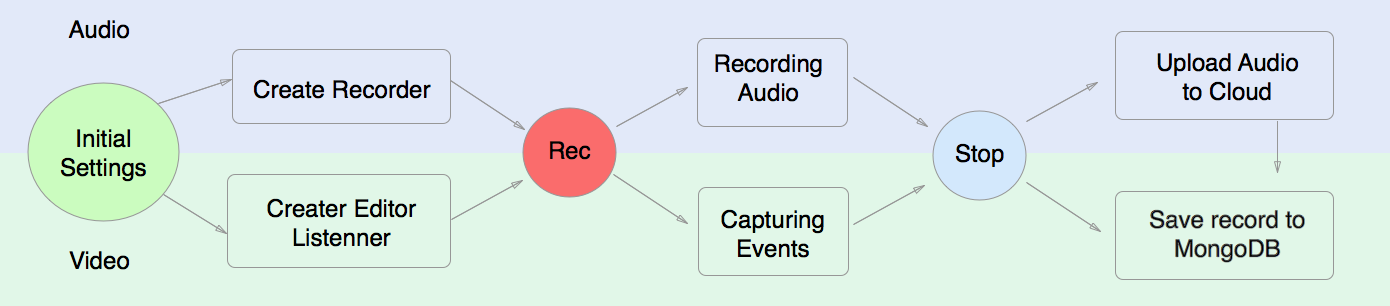
\includegraphics[width=1\textwidth]{recordProcess.png}
    	\label{fig:recProgress}
    }
    \subfigure[Proceso de reproducci�n]{
    	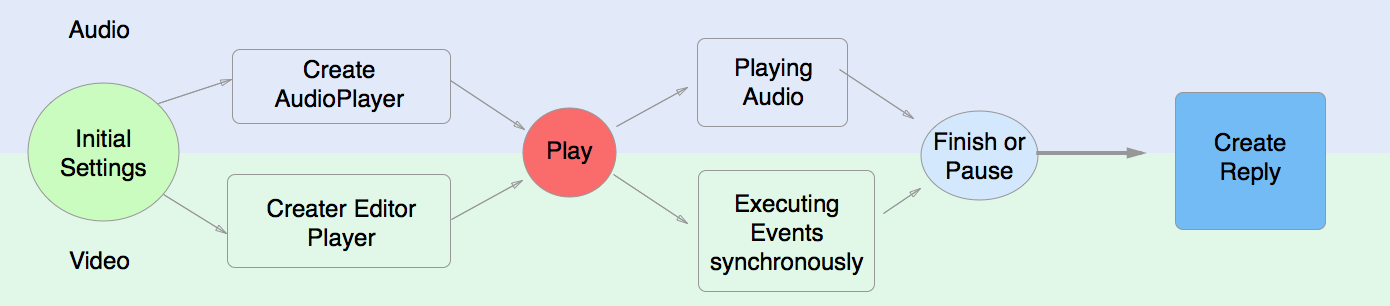
\includegraphics[width=1\textwidth]{playProcess.png}
	 \label{fig:playProgress}
    }
    \caption{Procesos de grabaci�n, reproducci�n y esquema de flujo.}
    \label{fig:processandflow}
\end{figure}
\paragraph{}
\section{Cloud Storage}
Necesitamos un servicio de almacenamiento de audio en la nube. Para ello hemos elegido el servicio de SoundCloud. SoundCloud nos proporciona una API REST muy sencilla de utilizar mediante su sdk. Esta nos permitir� subir archivos tipo blob que acabamos de grabar, crear un stream para una pista de audio concreta y borrar contenidos de manera limpia. Para utilizar su servicio es necesario la autenticaci�n del usuario y una aplicaci�n que crearemos en el espacio para desarrolladores de soundcloud. A esta aplicaci�n se le atribuir�n unos credenciales que permitir�n el acceso al API REST de SoundCloud. La configuraci�n de dicha aplicaci�n y el servicio dentro de nuestra plataforma se explicar� con m�s detalle en el cap�tulo \ref{cap:desarrollo}.

%%%%%%%%%%%%%%%%%%%%%%%%%%%%%%%%%%%%%%%%%%%%%%%%%%%%%%%%%%
%%%%%%%                  															       %%%%%%
%%%%%%%                               CAPITULO 4: DESARROLLO DE LA APLICACI�N                                %%%%%%
%%%%%%%  																	       %%%%%%
%%%%%%%%%%%%%%%%%%%%%%%%%%%%%%%%%%%%%%%%%%%%%%%%%%%%%%%%%%



\chapter{Desarrollo de la aplicaci�n}\label{cap:desarrollo}
\paragraph{}
El desarrollo de cualquier aplicaci�n viene despu�s de su dise�o. No necesariamente es el paso final, puesto que esta etapa sirve de feedback en el proceso general y muchas veces hay que retomar el dise�o para establecer nuevos requisitos o cambiar los actuales.
\section{Aprendizaje}
\paragraph{}
Una vez dise�ada la aplicaci�n y establecidas las herramientas a utilizar, el siguiente paso es profundizar en cada una de ellas. El aprendizaje de nuevas herramientas es lento pero el afianzamiento de los conocimientos necesarios de manera correcta nos evitar� muchos problemas en el futuro. Por esto hay que esforzarse en comprenderlos y la primera fase del Desarrollo de la aplicaci�n es el aprendizaje.



\subsection{CSS3 y preprocesadores}
Aqu� explicar� Qu� he aprendido de css3 y de los preprocesadores less y saas.
\subsection{API SoundCloud}
Aqu� explicar� el servicio de almacenamiento de SoundCloud.
\section{Componiendo el escenario}
Peque�a introducci�n
\subsection{Entorno de desarrollo}
WebStorm. Foto de la interfaz.
\subsection{Paquetes}
Lista de paquetes necesarios y sus funcionalidades
\subsection{Collecciones}
Explicar c�mo se han desarrollado las entidades en colecciones y la estructura de los objetos guardados. C�mo se relacionan.
\subsection{Enrutamiento}
Explicar Iron Router y su potencial.
\subsection{Mixins iniciales}
Foto de los mixines iniciales y que son necesarios.
\section{Layout Principal}
Estructura general de la vista de la aplicaci�n.
\section{Registro de usuarios}
Peque�a introduccion hablar de los servicios de meteor autom�ticos para sign.
\subsection{Sign In y Sign Up}
Funcionalidad y pantallas
\subsection{Verificaci�n de Email}
Funcionalidad y pantallas
\subsection{Cambio y recuperaci�n de contrase�a}
Funcionalidad y pantallas
\subsection{Servicios agregados}
Funcionalidad y pantallas.

\section{Sidebar}
Explicar que contenido se muestra en sidebar y que es el enlace a todos los recursos de la aplicaci�n desde cualquier pantalla.
\section{Formularios}
Peque�a introducci�n enumerar los formularios creados.
\subsection{Dise�o de plantilla din�mica}
Explicar c�mo se crea una plantilla din�mica para los formularios.
\subsection{Creadores de entidades}
Enumerarlos y pantallas.
\subsection{Conversaciones}
Hablar del componente inputMembers.
\subsection{Grabaciones}
Hablar del grabador. (extenso).

\section{Entidades}
Hay que dar forma a las entidades visualmente.
\subsection{Canales}
Hablar de los canales.
\subsection{Lecciones}
Hablar de las lecciones.
\subsection{Secciones}
Hablar de las secciones.
\subsection{Grabaciones}
Hablar de la reproducci�n de las grabaciones. (extenso)
\subsection{Listas de reproducci�n}
Asociadas a una secci�n.
\subsection{Conversaciones}
Hablar de las conversaciones y de los roles.
\section{Perfil de usuario}
\subsection{Rol due�o}
\subsection{Rol visitante}
\subsection{Contactos}
\section{Tutoriales}
\section{Landing}
\section{BrowseCrossing}
\section{Full Responsive}
\section{Despliegue}
\chapter{Pruebas de Validaci�n}
En este cap�tulo se representa la fase de experimentaci�n del proyecto. Esta fase se basa en la realizaci�n de una prueba en la que se ha medido la utilidad de la aplicaci�n y su rendimiento en un entorno real.
\section{Motivaci�n}
La principal motivaci�n de este experimento es analizar el comportamiento de la aplicaci�n en la realidad. Dicho comportamiento deber� cumplir estrictamente los requisitos propuestos en la secci�n \ref{sec:requisitos}.
\section{Planteamiento y objetivos}
Una vez desplegada la aplicaci�n en Heroku \cite{baz14} y realizadas las pruebas globales oportunas se ha procedido a generar contenido en la misma y a plantear el experimento. 
\paragraph{}
El experimento consistir� en hacer accesible la aplicaci�n a un grupo de alumnos mediante la difusi�n de la url donde ha sido alojada. Dichos alumnos, siguiendo la gu�a de uso elaborada para esta fase del proyecto, explotar�n todas las caracter�sticas de la aplicaci�n y su funcionalidad. Por otra parte se ha integrado a la aplicaci�n el servicio de Google Analytics \footnote{\url{https://analytics.google.com}} para controlar y analizar el flujo de usuarios dentro de la aplicaci�n.
\paragraph{}
Los objetivos perseguidos se han resumido en las siguientes caracter�sticas:
\begin{itemize}
	\item \textbf{Funcional:} la aplicaci�n debe cumplir todos los requisitos establecidos.
	\item \textbf{Atractiva e intuitiva:} que los alumnos aprecien el atractivo de las interfaces y el flujo de la aplicaci�n.
	\item \textbf{Fluida y �ptima:} la aplicaci�n debe comportarse de manera fluida con m�s de un usuario utiliz�ndola.
	\item \textbf{�til:} la aplicaci�n debe suponer una herramienta de trabajo para los alumnos. 
\end{itemize}
\paragraph{}
Para medir y analizar el cumplimiento de los objetivos marcados se ha desarrollado una encuesta o formulario que se ha difundido junto con la gu�a de uso. Los alumnos, una vez completada la gu�a, aportar�n informaci�n sobre su experiencia contestando a las preguntas de dicho formulario.
\section{Proceso y realizaci�n}
El proceso y la realizaci�n ha sido muy sencilla, Se han habilitado los recursos necesarios (gu�a y formulario) de forma remota y se ha procedido al env�o de dichos enlaces a un grupo de alumnos.
\section{Resultados y an�lisis}
Una vez que los alumnos han probado la aplicaci�n y han rellenado la encuesta se ha procedido al an�lisis de los resultados. 
\chapter{Conclusi�n}
\phantomsection
%% cite example: \cite{baz1}%%
\addcontentsline{toc}{chapter}{\bibname}
\begin{thebibliography}{99}
	\bibitem{baz1} P�gina oficial WebRTC: \url{https://webrtc.org/}
	\bibitem{baz2} P�gina para WebRTC experiments (recordRTC): \url{https://www.webrtc-experiment.com/RecordRTC/}
	\bibitem{AceEditor} P�gina oficial de AceEditor: \url{https://ace.c9.io/}
	\bibitem{AceEditorPackage} Paquete AceEditor para Meteor: \url{https://github.com/mizzao/meteor-sharejs}
	\bibitem{baz3} P�gina oficial SoundCloud: \url{https://soundcloud.com}
	\bibitem{baz4} P�gina para desarrolladores SoundCloud: \url{https://developers.soundcloud.com/}
	\bibitem{baz5} P�gina oficial MeteorJS: \url{https://www.meteor.com/}
	\bibitem{baz6} Gu�a de MeteorJS: \url{http://guide.meteor.com/}
	\bibitem{baz7} Documentaci�n de MeteorJS: \url{http://docs.meteor.com/#/full/}
	\bibitem{bazMongoDB} P�gina oficial de MongoDB: \url{https://www.mongodb.com/es}
	\bibitem{baz8} P�gina oficial Bootstrap: \url{http://getbootstrap.com/}
	\bibitem{baz9} W3C javascript tutorial: \url{http://www.w3schools.com/js/}
	\bibitem{baz10} Documentaci�n de MongoDB: \url{https://docs.mongodb.com/manual/}
	\bibitem{baz11} P�gina oficial JQuery: \url{https://jquery.com/}
	\bibitem{baz12} Documentaci�n de JQuery: \url{http://api.jquery.com/}
	\bibitem{baz13} Documentaci�n de UnderscoreJS: \url{http://underscorejs.org/}
	\bibitem{bazIronRouter} Repositorio de Iron Router en Github: \url{https://github.com/iron-meteor/iron-router}
	\bibitem{baz14} Despliegue en Heroku: \url{https:duckflight.herokuapp.com/}
	\bibitem{bazGitRepo} C�digo fuente del proyecto: \url{https://github.com/jortegamo/duckflight}
	\bibitem{bazWikiProyect} Wiki del proyecto: \url{https://github.com/jortegamo/duckflight/wiki}
	\bibitem{bazWikiTutoriales} Documentaci�n del producto: \url{https://github.com/jortegamo/duckflight/wiki/Video-Tutoriales}
	\bibitem{bazHeroku} Tutorial para el despliegue: \url{http://justmeteor.com/blog/deploy-to-production-on-heroku/}
	\end{thebibliography}

\appendix
\clearpage 
\addappheadtotoc
\appendixpage
\chapter{Dise�o de la base de datos y documentos para MongoDB}
En este ap�ndice se muestra el esquema Entidad Relaci�n y los objetos BSON dise�ados para cada una de las entidades.
\label{appendix:documentsdesign}
\begin{figure}[htpb]
	\centering
	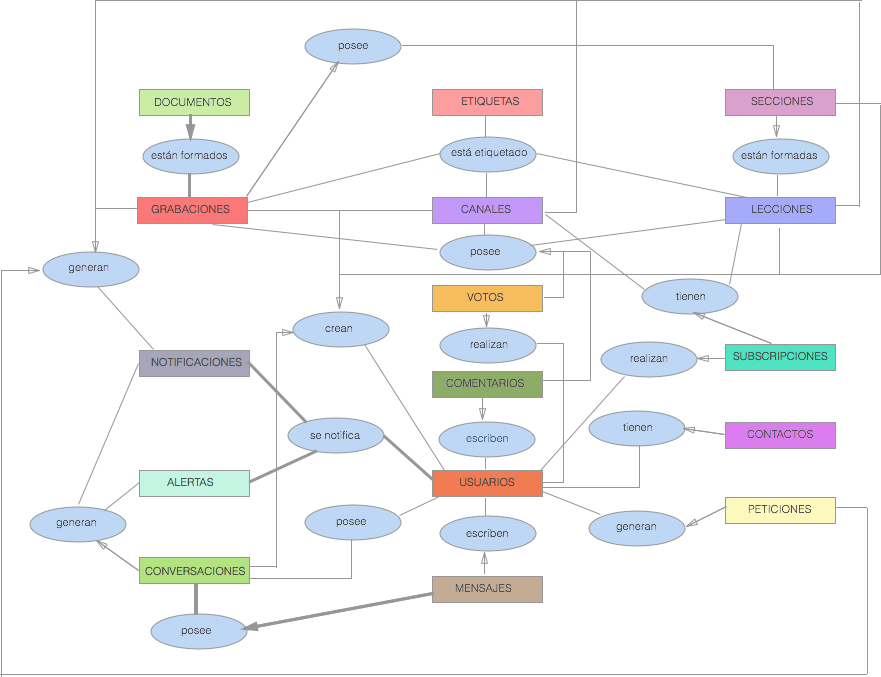
\includegraphics[width=0.9\textwidth]{ERdesign.png}
	\caption{Esquema entidad relaci�n}
	\label{fig:ERdesign}
\end{figure}
\vspace{1cm}
\begin{lstlisting}[language=javascript, caption=Dise�o de documento para una grabaci�n, label={recordMongo}]
var record = {
    _id: //idMongo,
    author: //idUser,
    title: //no �nico,
    description: //(opcional),
    RC: [{},...], //Funciones de reproducci�n sobre el editor
    createAt: //fechaCreaci�n,
    docs_count: //contador de documentos,
    votes_count: //contador de votos,
    replies_count: //contador de respuestas,
    comments_count: //contador de comentarios,
    channel_id: //canal al que pertenece,
    lesson_id: //lecci�n a la que pertenece,
    section_id: //secci�n a la que pertenece dentro de una lecci�n,
    order: ,//orden dentro de la lista de reproducci�n.
    tags: [{},...], //etiquetas,
    ready: //(boolean) para conocer la disponibilidad del record.
    img: //imagen miniatura,
    duration: //duraci�n en milisegundos de la grabaci�n.
    isReply: //(boolean) indica si se trata de una respuesta a otro record.
    parent_id: //idMongo del record al que responde.
    track: //{_id: 'id del track en SoundCloud', link: 'link SoundCloud'}
}; 
\end{lstlisting}
\vspace{1cm}
\begin{lstlisting}[caption=Dise�o de documento para los documentos de cada grabaci�n, label={documentMongo}]
var doc = {
    _id: //idMongo,
    record: //record al que pertenecen,
    doc: {
         title: //titulo del documento (�nico para el record),
         theme: //tema del editor tras �ltimo cambio,
         mode: //tema del editor tras el �ltimo cambio,
         value: //�ltimo estado del contenido del editor
    },
    start: //(boolean) (True)? comienzo grabaci�n : se ha creado durante la grabaci�n
           //o es el estado final de otro inicial.
};

\end{lstlisting}
\vspace{1cm}
\begin{lstlisting}[caption=Dise�o de documento para un canal, label={channelMongo}]
var channel = {
    _id: //idMongo,
    author: //id_user,
    title: //�nico,
    banner: //url img banner,
    img: //url img miniatura,
    description: //(opcional),
    tags: //etiquetas [{name: //nombre etiqueta}],
    createAt: //fechaCreaci�n,
    votes_count: //contador para los votos,
    records_count: //contador para los records,
    comments_count: //contador para los comentarios,
    users_count: //contador para los usuarios que se subscriban
};
\end{lstlisting}
\vspace{1cm}
\begin{lstlisting}[caption=Dise�o de documento para una lecci�n, label={lessonMongo}]
var lesson = {
    _id: //idMongo,
    author: //id_user,
    title: //�nico,
    img: //url img miniatura,
    description: //(opcional),
    tags: //etiquetas [{name: //nombre etiqueta}],
    createAt: //fechaCreaci�n,
    votes_count: //contador para los votos,
    sections_count: //contador para las secciones,
    comments_count: //contador para los comentarios,
    users_count: //contador para los usuarios que se apunten
}; 
\end{lstlisting}
\vspace{1cm}
\begin{lstlisting}[caption=Dise�o de documento para una secci�n, label={sectionMongo}]
var section = {
    _id: //idMongo,
    title: //�nico,
    createAt: //fechaCreaci�n,
    records_count: //contador para los records,
    lesson_id: //id de la lecci�n a la que pertenece.
    order: //orden de la secci�n.
}; 
\end{lstlisting}
\vspace{1cm}		
\begin{lstlisting}[caption=Dise�o de documento para cada subscripci�n de un usuario, label={userEnrolledMongo}]
var userEnrolled = {
    _id: //idMongo,
    contextId: //id del canal o de la lecci�n a la que se han subscrito,
    user_id: //id del usuario
};
\end{lstlisting}
\vspace{1cm}
\begin{lstlisting}[caption=Dise�o de documento para una etiqueta, label={tagMongo}]
var tag = {
    _id: //idMongo,
    name: //nombre para la etiqueta
};
\end{lstlisting}
\vspace{1cm}
\begin{lstlisting}[caption=Dise�o de documento para una conversaci�n, label={conversationMongo}]
var conversation = {
    _id: //idMongo,
    subject: //asunto de la conversaci�n,
    author: //l�der de la conversaci�n.
    last_modified: //fecha de ultima modificaci�n (cada vez que se inserta un mensaje),
    members: //[{},...], array de miembros,
    members_count: //contador para los miembros,
    messages_count: //contador para los mensajes
};
\end{lstlisting}
\vspace{1cm}
\begin{lstlisting}[caption=Dise�o de documento para los mensajes, label={messageMongo}]
var message = {
    _id: //idMongo,
    author: //id del creador,
    createdAt: //fecha de creaci�n,
    message: //contenido del mensaje
    conversation_id: //id de la conversaci�n a la que pertenece.
}
\end{lstlisting}
\vspace{1cm}
\begin{lstlisting}[caption=Dise�o de documento para una alerta de conversaci�n, label={conversationAlertMongo}]
var conversationAlert = {
    _id: //idMongo,
    user_id: //usuario al que se le muestra la alerta,
    conversation_id: //id de la conversaci�n de la que procede,
    alertsAllow: //flag (boolean) si es true se muestran las alertas y si es false no.
    alerts_count: //contador de alertas
};
\end{lstlisting}
\vspace{1cm}
\begin{lstlisting}[caption=Dise�o de documento para cada usuario, label={userMongo}]
var user = {
    _id: //idMongo,
    username: //nombre de usuario (�nico),
    avatar: //avatar del usuario,
    banner: //banner de la pagina de usuario,
    description: //descripci�n del usuario,
    status: //estado de conexi�n,
    emails: //[{address: //emailAddress,verified: //Boolean,},...],
    ... //otros campos establecidos por meteor-accounts.
};
\end{lstlisting}
\vspace{1cm}
\begin{lstlisting}[caption=Dise�o de documento para las peticiones de contacto, label={requestsMongo}]
var request = {
    _id: //idMongo,
    requested: //{id: id_user, delete: boolean},
    applicant: //{id: id_user, delete: boolean},
    status: //(string) 'pending', 'accepted', 'refused'
};
\end{lstlisting}
\vspace{1cm}
\begin{lstlisting}[caption=Dise�o de documento para establecer la relaci�n de contacto, label={relationMongo}]
var relation = {
    _id: //idMongo,
    createdAt: //fecha creaci�n,
    users: //[id_user_requested, id_user_applicant],
};
\end{lstlisting}
\vspace{1cm}
\begin{lstlisting}[caption=Dise�o de documento para los comentarios, label={commentMongo}]
var comment = {
    _id: //idMongo,
    author: //id del creador,
    createdAt: //fecha de creaci�n,
    isReply: //(Boolean) indica si es una respuesta o no,
    replies_count: //contador de respuestas,
    message: //contenido del mensaje
};
\end{lstlisting}
\vspace{1cm}
\begin{lstlisting}[caption=Dise�o de documento para una notificaci�n, label={notificationMongo}]
var notification = {
    _id: //idMongo,
    to: //id_user destinatario,
    from: //id_user origen,
    parentContextTitle: //es el t�tulo de la lecci�n, record o channel en el que se ha producido,
    urlParameters: //son los par�metros para construir el enlace al clickar sobre la notificaci�n,
    type: //(string) 'channel', 'record', 'comment', etc,
    message: //(string) de contenido HTML
};
\end{lstlisting}










\end{document}  


